%%%%%%%%%%%%%%%%%%%%%%%%%%%%%%%%%%%%%%%%%%%%%%%%%%%%%%
%% Fleet dynamics models in FLBEIA
%%%%%%%%%%%%%%%%%%%%%%%%%%%%%%%%%%%%%%%%%%%%%%%%%%%%%%

\documentclass[12pt, halfline, a4paper]{ouparticle}

\usepackage[utf8]{inputenc}
\usepackage{lscape}
\usepackage{rotating}
\usepackage{booktabs}
\usepackage{longtable}
\usepackage{subfigure}
%%%%%%%%%%%%%%%%%%%%%%%%%%%%%%%%%%%%
\begin{document}

\title{Working title: Integrating location choice models in mixed-fishery
	management strategy evaluations}

\author{
	\name{Paul J. Dolder}
	\address{GMIT}
	\email{paul.dolder@research.gmit.ie}
	\address{CEFAS}
	\email{paul.dolder@cefas.co.uk\thanks{Corresponding author} }
	\and
	\name{Cóilín Minto}
	\address{GMIT}
	\email{coilin.minto@gmit.ie}
	\and
	\name{Dorleta Garcia}
	\address{AZTI}
	\email{dgarcia@azti.es}
}

\abstract{Some text here}

\date{\today}

\keywords{MSE, mixed fisheries, fleet dynamics, RUM, Markov}

\maketitle

\section{Introduction}
\label{intro}

Most fisheries worldwide are mixed. Evaluation of management performance is
still based on single-species, failing to take account of fleet dynamics;
technical (mixed-fishery) interactions affect the outcome of management
measures through either discarding unwanted catch or ``choking" of quota when
first limit reached. It's important for MSEs to take account of these
interactions when evaluating management strategies in order to move towards a
more holistic approach to fisheries management.  \\

In order to address this mixed fishery methods have been developed and applied
to numerous case studies (REFs). The mixed-fishery approach models activity of
fleets (vessels of similar physical characteristic) and how the deployment of
fishing effort in different métier (activity defined by similar catch patterns)
contribute to catch of multiple stocks simultaneously. The assumption about the
amount of fishing effort deployed in each of the métier and stability of
catchability for the different stocks determines the outcome for the fishery in
terms of fishing mortality and catch for each stock. The sum of the different
fleets activity (and their catch composition and selectivity) thus provides a
different picture on exploitation of stocks exploited concurrently. \\ 

A limitation in evaluated management strategies from a mixed fishery
perspective is the lack of operating model to account for how fisher behaviour
affects catch of multiple stocks. Location choice is one key decision that
effects catch in mixed fisheries. Different locations have different density of
target and non-target species, therefore choice of where to fish determines how
much of each species caught. This is rarely taken into account in simulations
of management strategies.\\

FLBEIA is a full feedback Management Strategy Evaluation framework that can be
used to take account of mixed-fishery interactions when evaluating different
harvest rules, modelling selectivity improvements and biological and economic
aspects of fisheries. FLBEIA takes a modular approach to modelling
mixed-fisheries, with components for biological and fleet operating models,
management procedures and can take account of full feedback and uncertainty in
management outcome [Insert general diagram of FLBEIA structure]. Generally
applications assume constant fleet dynamics (REFs), with exploitation per unit
of effort for different fleets remaining static inter-annually. This limits
understanding of the impact of fleet dynamics on outcomes for different
fisheries strategies. \\

Here, we extend application of FLBEIA to include commonly used fleet dynamics
models for location choice. This includes the Caddy Gravity model, the
conditional logit Random Utility model and a Markov transition model. We apply
the models to the Celtic Sea demersal fisheries, with location choice for Irish
otter trawlers among nine areas determined by each of the location choice
models and compared to a base case of constant effort. In doing so we show how
different outcomes may be achieved given different assumptions about location
choice. We recommend implementation of different fleet location choice
operating models when undertaking mixed-fishery MSEs in order to incorporate
this important dynamic alongside plausible biological dynamics to better
characterise outcomes for fisheries indicators. \\


\section{Methods}
\label{meth}

\begin{itemize}
	\item Implementation of fleet dynamics models in FLBEIA (pseudo-code)
	\item Conditioning of seasonal FLBEIA model
		\begin{itemize}
			\item 4 seasons
			\item Metiers defined by spatial patterns in catch
			\item Implement fleet dynamics model for Irish otter
				trawlers
		\end{itemize}
	\item Fitting of models 
		\begin{itemize}
			\item Gravity
			\item Gravity + tradition
			\item RUM
			\item Markov 
			\item Model selection for RUM and Markov.
		\end{itemize}
	\item Simulations including closures
		\begin{itemize}
			\item Close a metier, how does effect reallocate
		\end{itemize}
	\item MSE with different fleet dynamics models as OM
\end{itemize}

\section{Results}
\label{res}

Characteristics of the different modelling approaches. \\

How each model is affecting by different species catch rates \\.

Combining inference from the models (different location choice OM, conclusions
about overall strategy. \\


\section{Discussion}
\label{dis}

\section{Conclusions}
\label{con}


\begin{notes}[Acknowledgements]
The authors would like to thank...
\end{notes}

\begin{thebibliography}
ggg
\end{thebibliography}

\newpage

\begin{table}
	\center
	\begin{tabular}{p{4cm} p{3cm} p{2cm} p{2cm} p{2cm}}
		\toprule
		Stock & Code & Fmsy & Blim & Bmsytrigger \\
		\hline
		Cod & COD & 0.35 & 7,300  & 10,300 \\
		Haddock & HAD & 0.4 & 6,700 & 10,000 \\
		Anglerfishes & ANF/MON & 0.28 & 16,032 & 22,278 \\
		European Hake & HKE & 0.28 & 32,000 & 45,000 \\
		Megrims & LEZ/NMEG & 0.191 & 37,100 & 41,800 \\
		Whiting & WHG & 0.52 & 25,000 & 35,000 \\
		\textit{Nephrops} FU16 & NEP16 & 0.062 & 19,880 & 49,700 \\
		\textit{Nephrops} FU17 & NEP17 & 0.085 & 4,637 & 11,593 \\
	        \textit{Nephrops} FU19 & NEP19 & 0.093 & 4,032 & 10,080 \\
		\textit{Nephrops} FU2021 & NEP2021 & 0.06 & 33,040 & 82,600 \\
		\textit{Nephrops} FU22 & NEP22 & 0.128 & 7,585 & 18,963 \\
		\bottomrule
	\end{tabular}
	\label{tab:brp}
	\caption{Biological Reference Points used in the Harvest Control Rules for each
		stock when setting the overall annual Total Allowable Catch.}
\end{table}

\newpage

\begin{figure}[!ht]
	\centering
	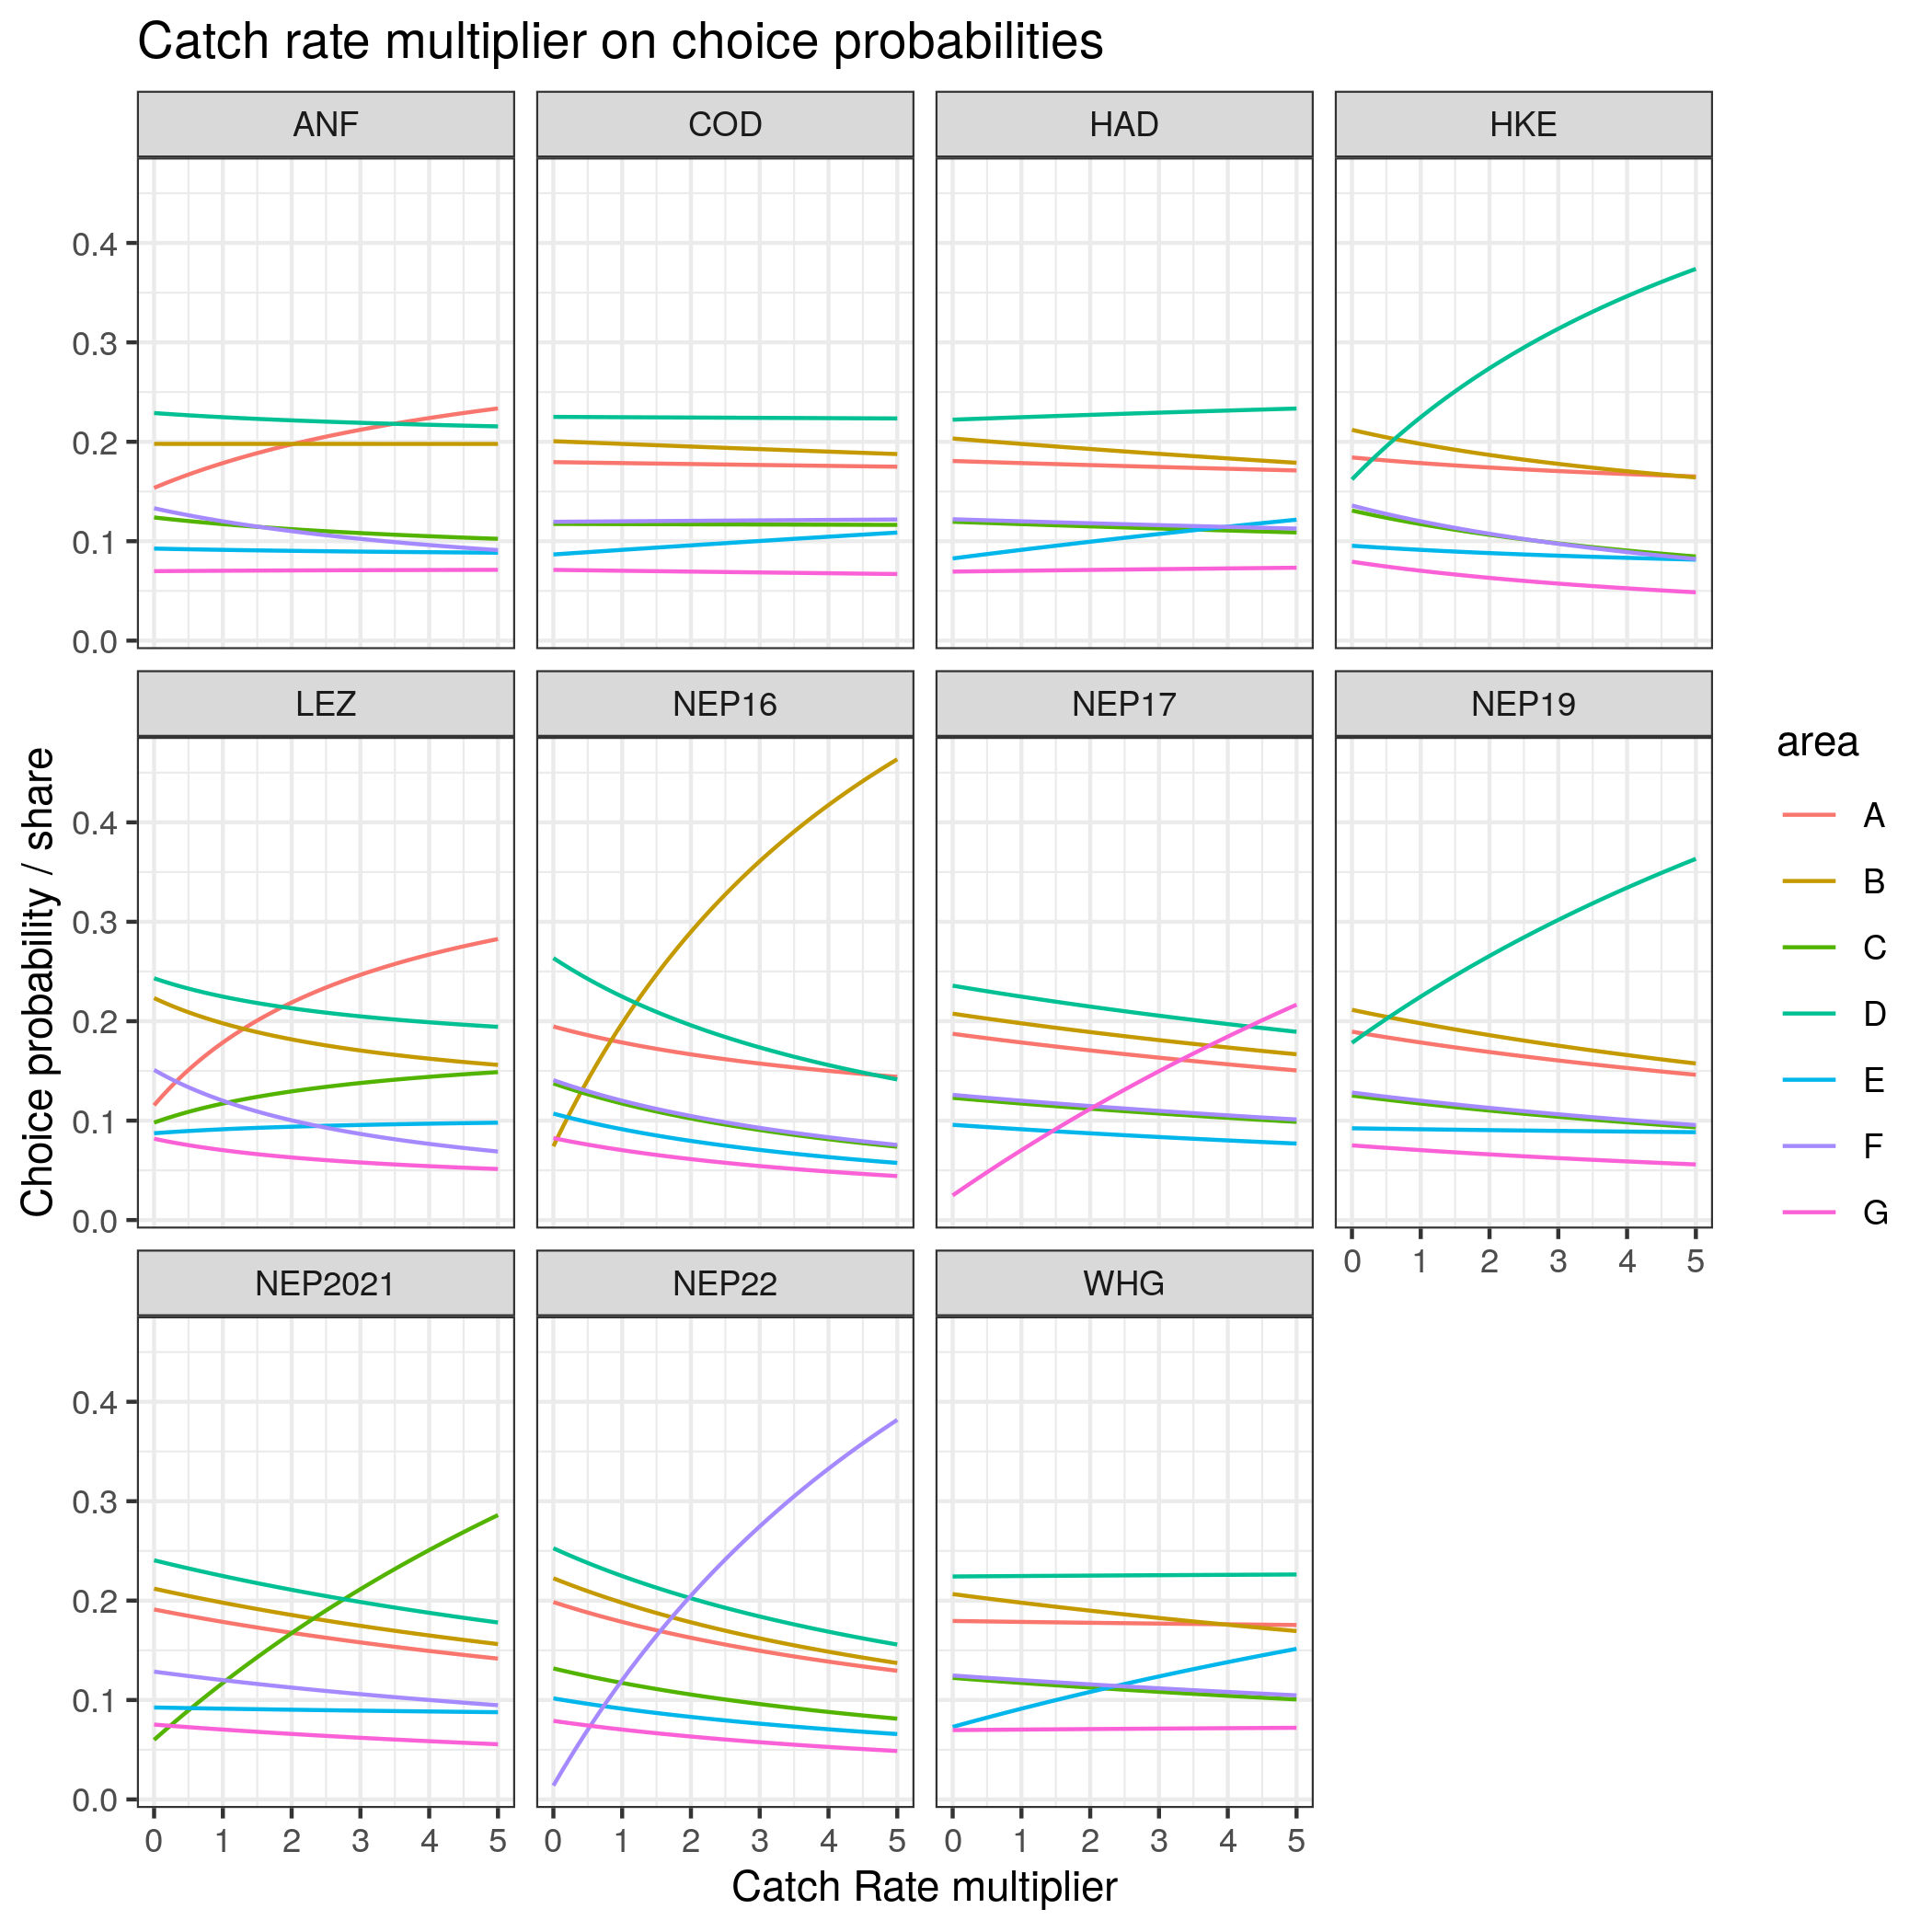
\includegraphics[width=1\linewidth]{figures/Gravity_Metier_Catch_Rate_Multiplier}
	\caption{The influence of changes in catch rates of different stocks on
	effort allocation among métier from the Gravity model.} 
	\label{fig:Grav_CR}
\end{figure}	

\begin{figure}[!ht]
	\centering
	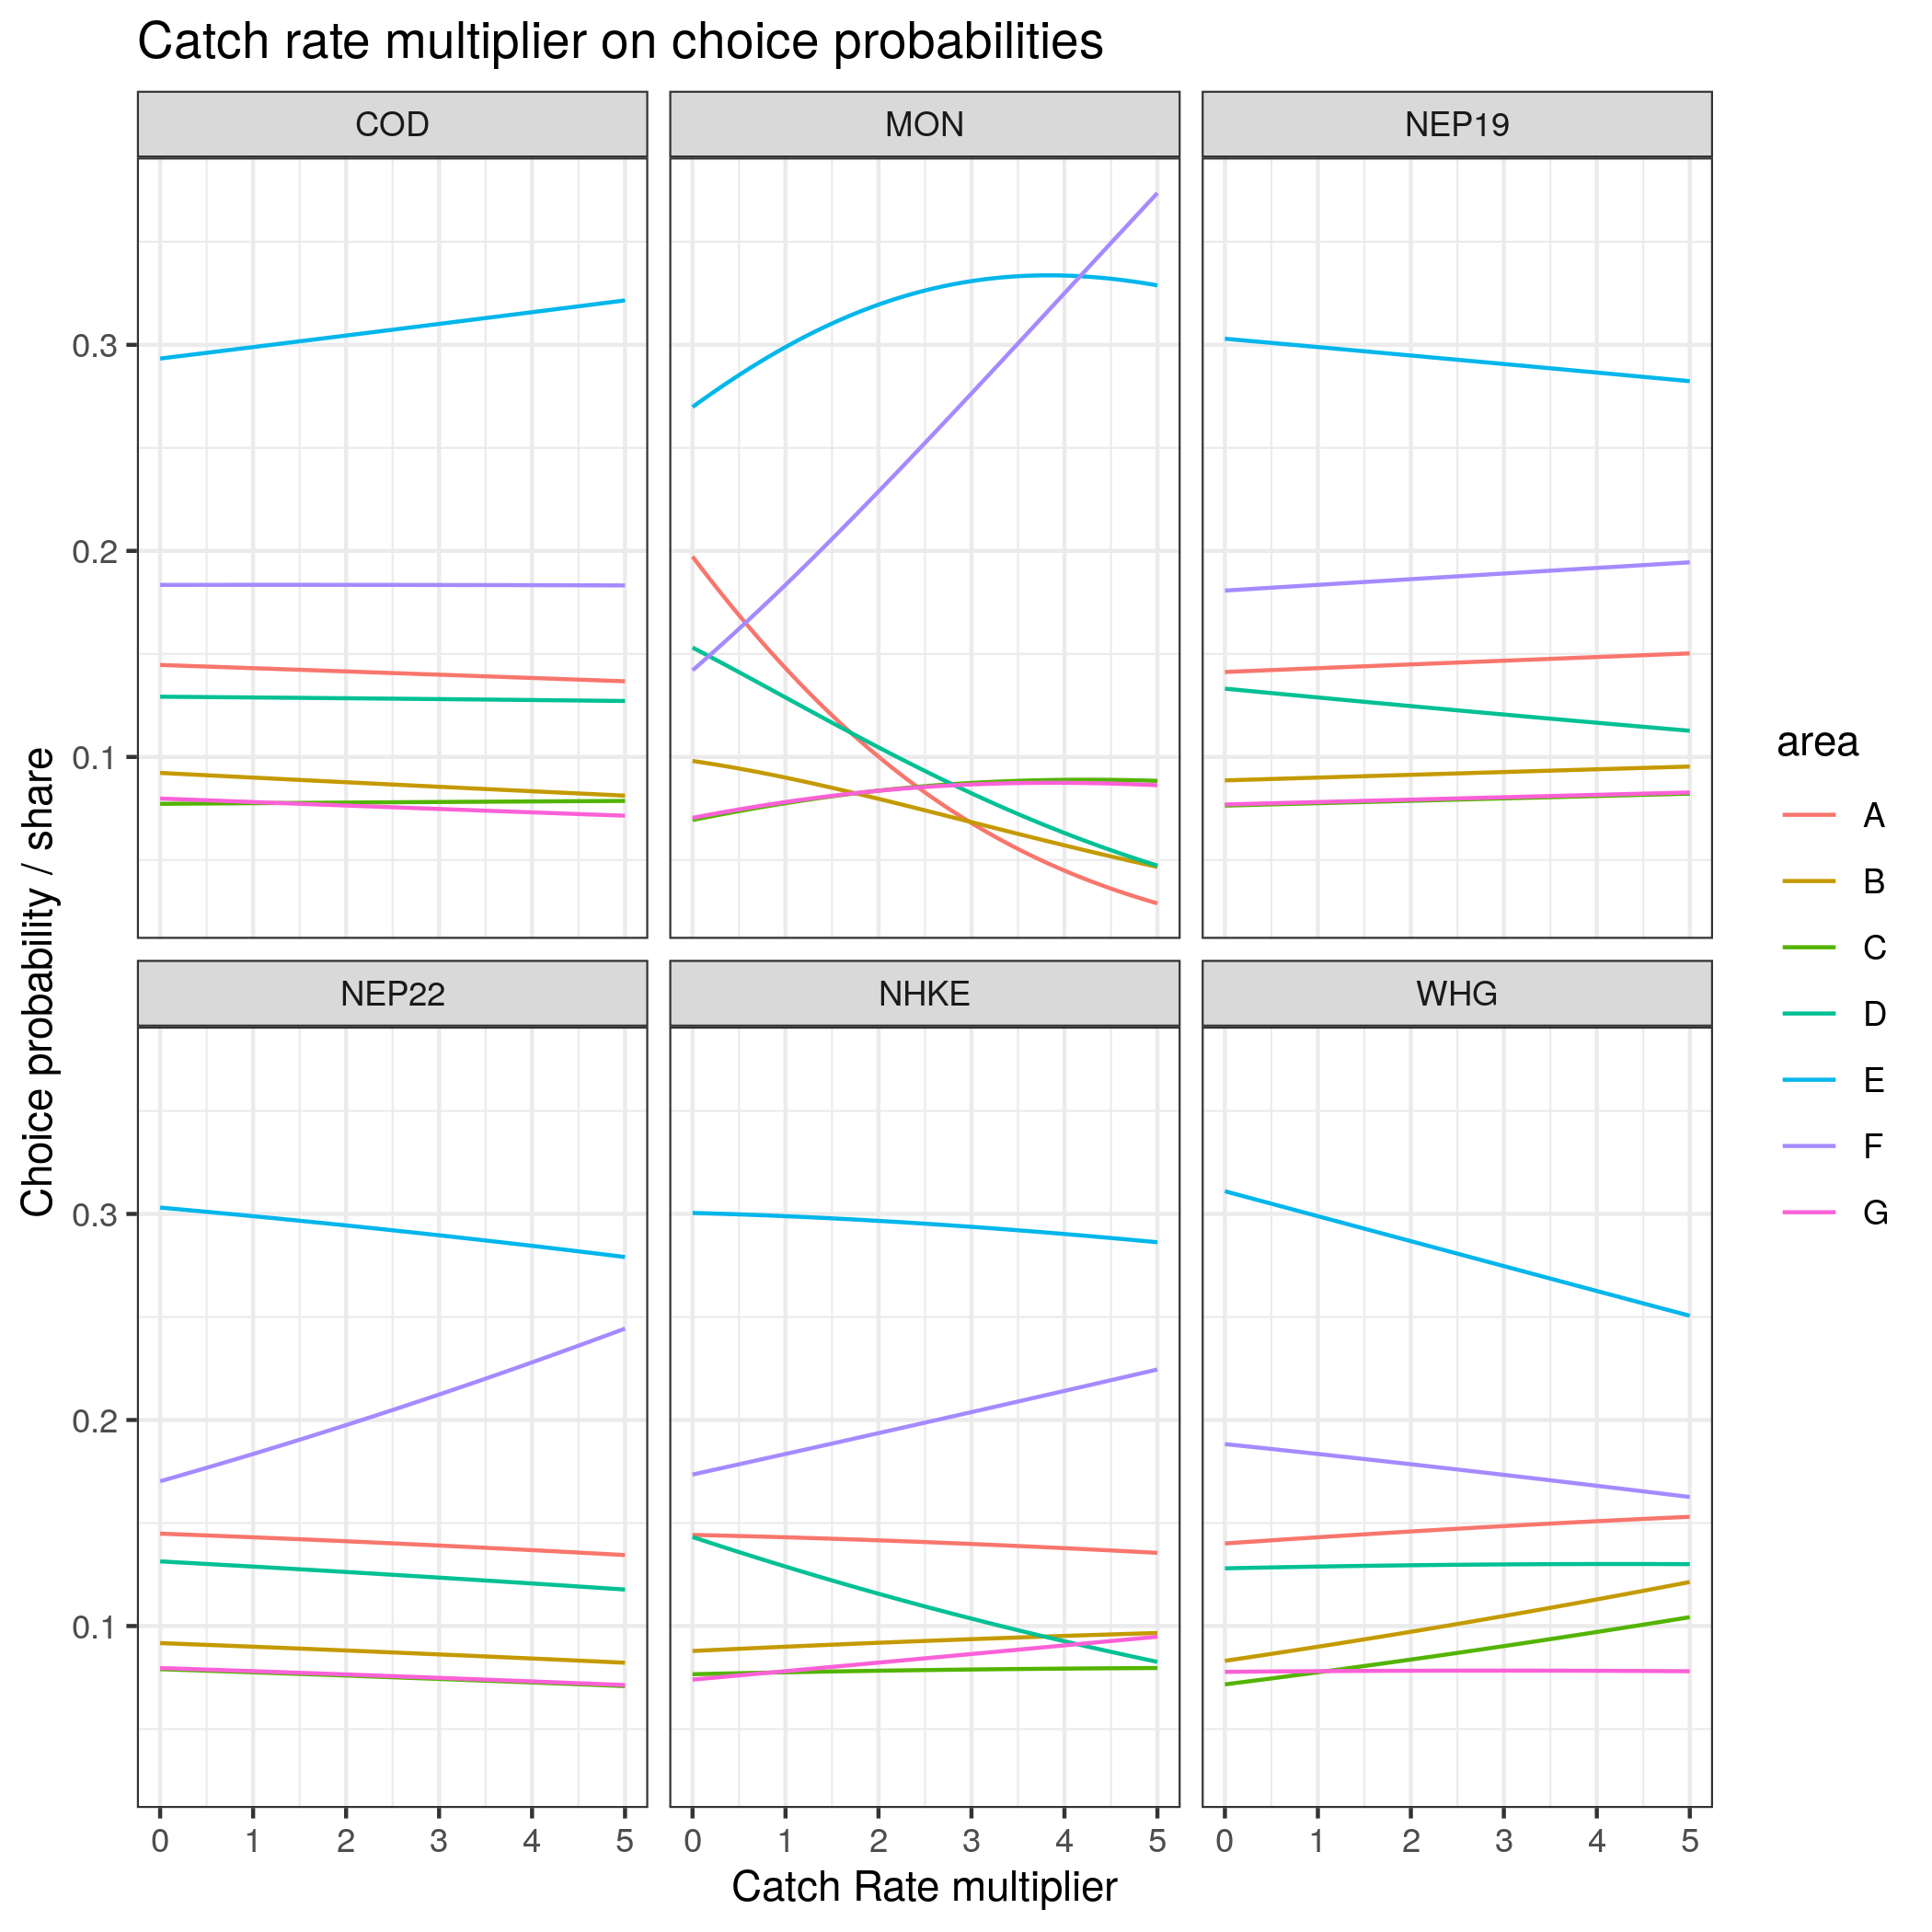
\includegraphics[width=1\linewidth]{figures/RUM_Metier_Catch_Rate_Multiplier}
	\caption{The influence of changes in catch rates of different stocks on
	effort allocation among métier from the RUM.} 
	\label{fig:RUM_CR}
\end{figure}	

\begin{figure}[!ht]
	\centering
	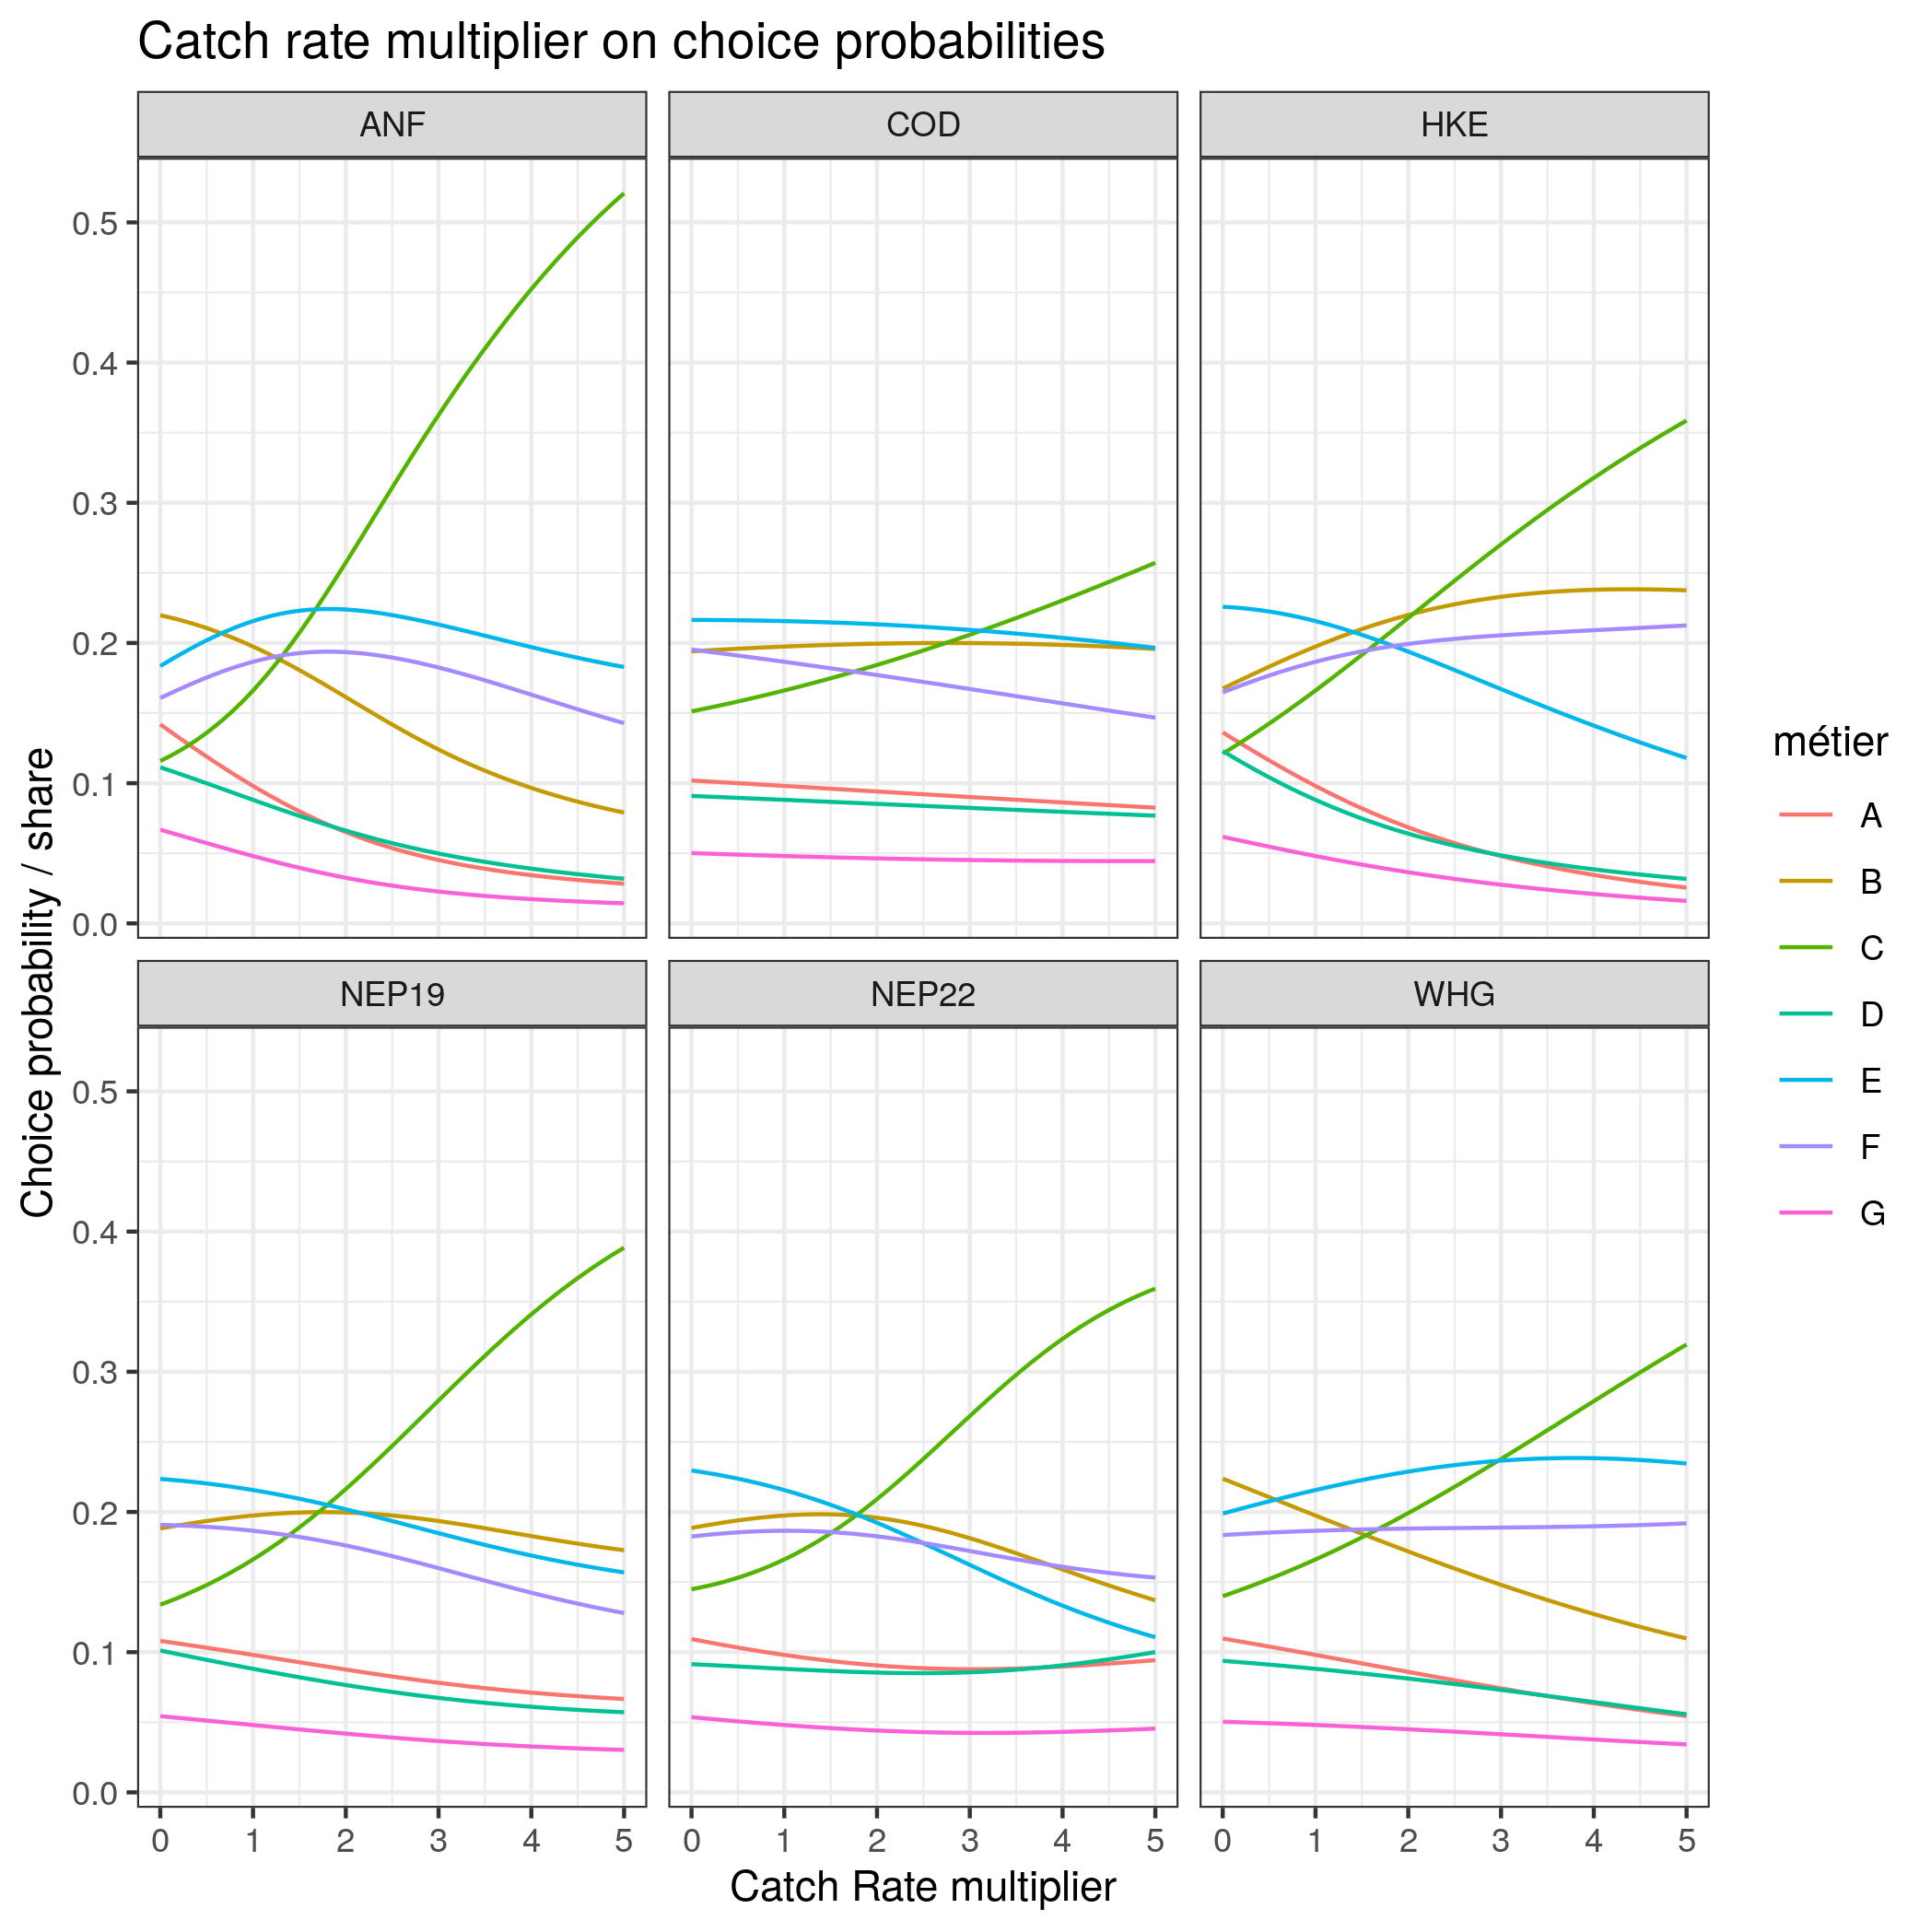
\includegraphics[width=1\linewidth]{figures/Markov_Metier_Catch_Rate_Multiplier}
	\caption{The influence of changes in catch rates of different stocks on
	effort allocation among métier from the Markov model.} 
	\label{fig:Markov_CR}
\end{figure}	

\begin{figure}[!ht]
	\centering
	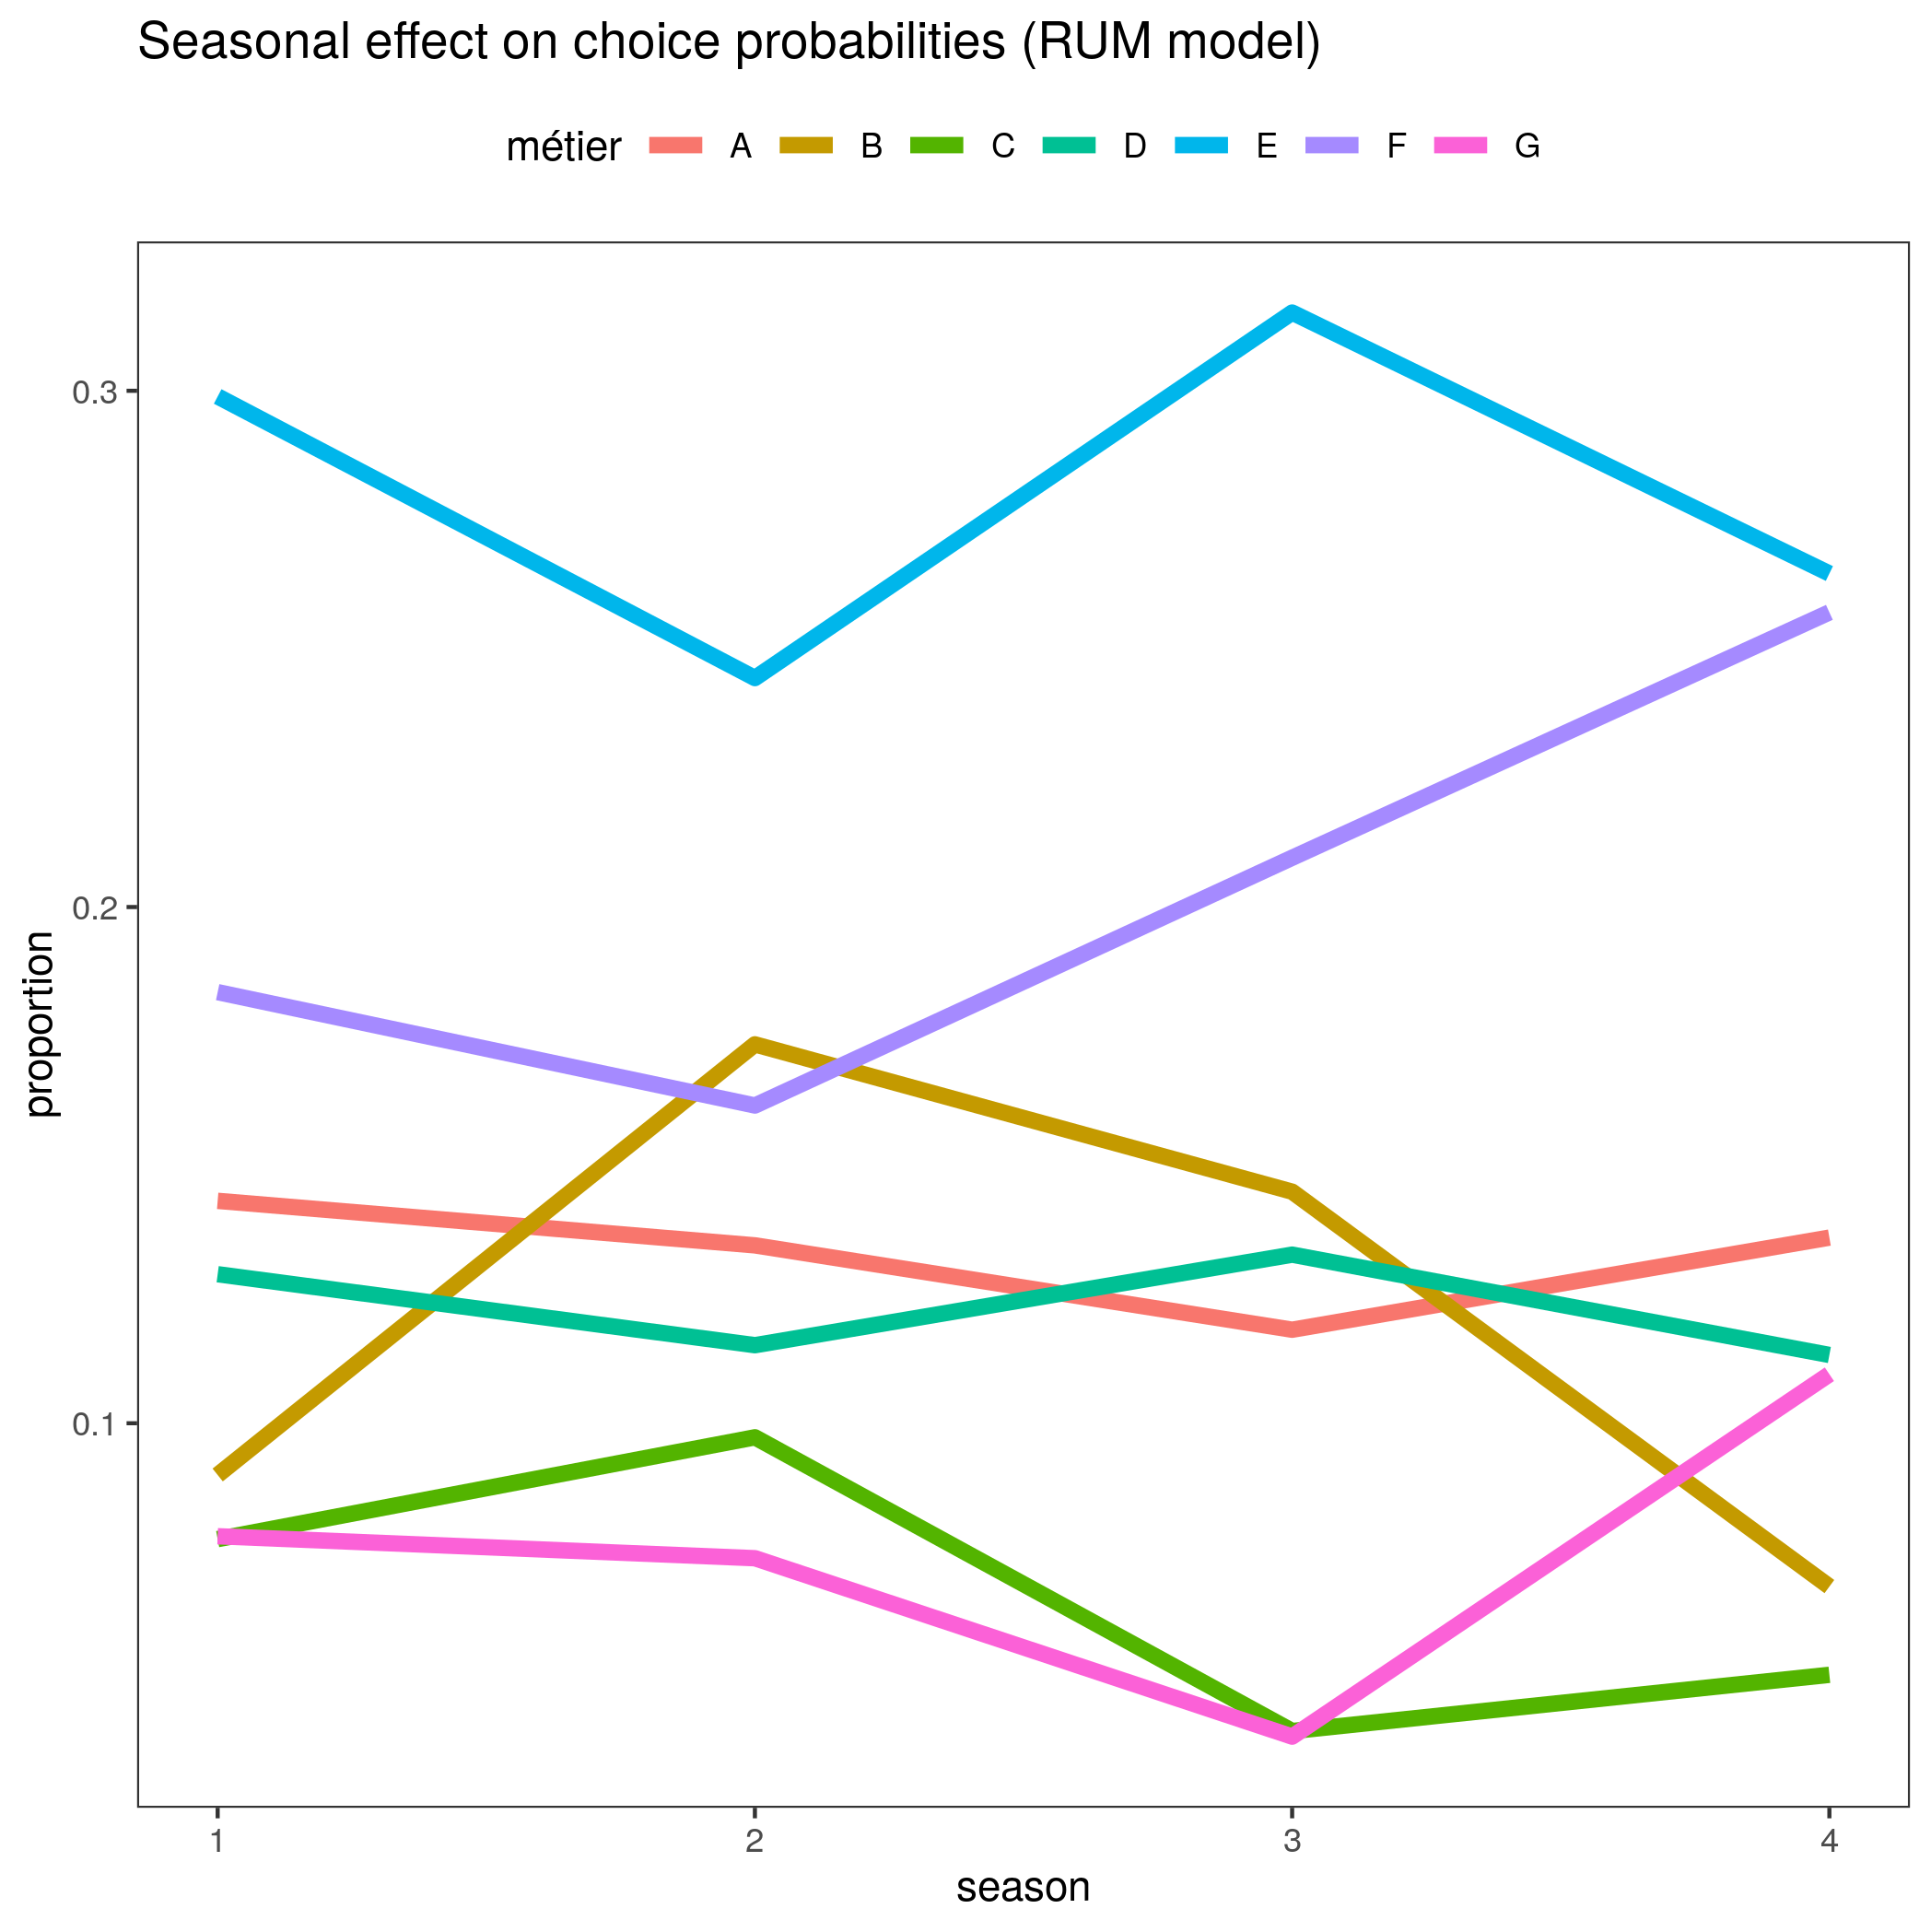
\includegraphics[width=1\linewidth]{figures/RUM_metier_seasonal_effect}
	\caption{Seasonal effect in the RUM model.} 
	\label{fig:RUM_Seas}
\end{figure}	

\begin{figure}[!ht]
	\centering
	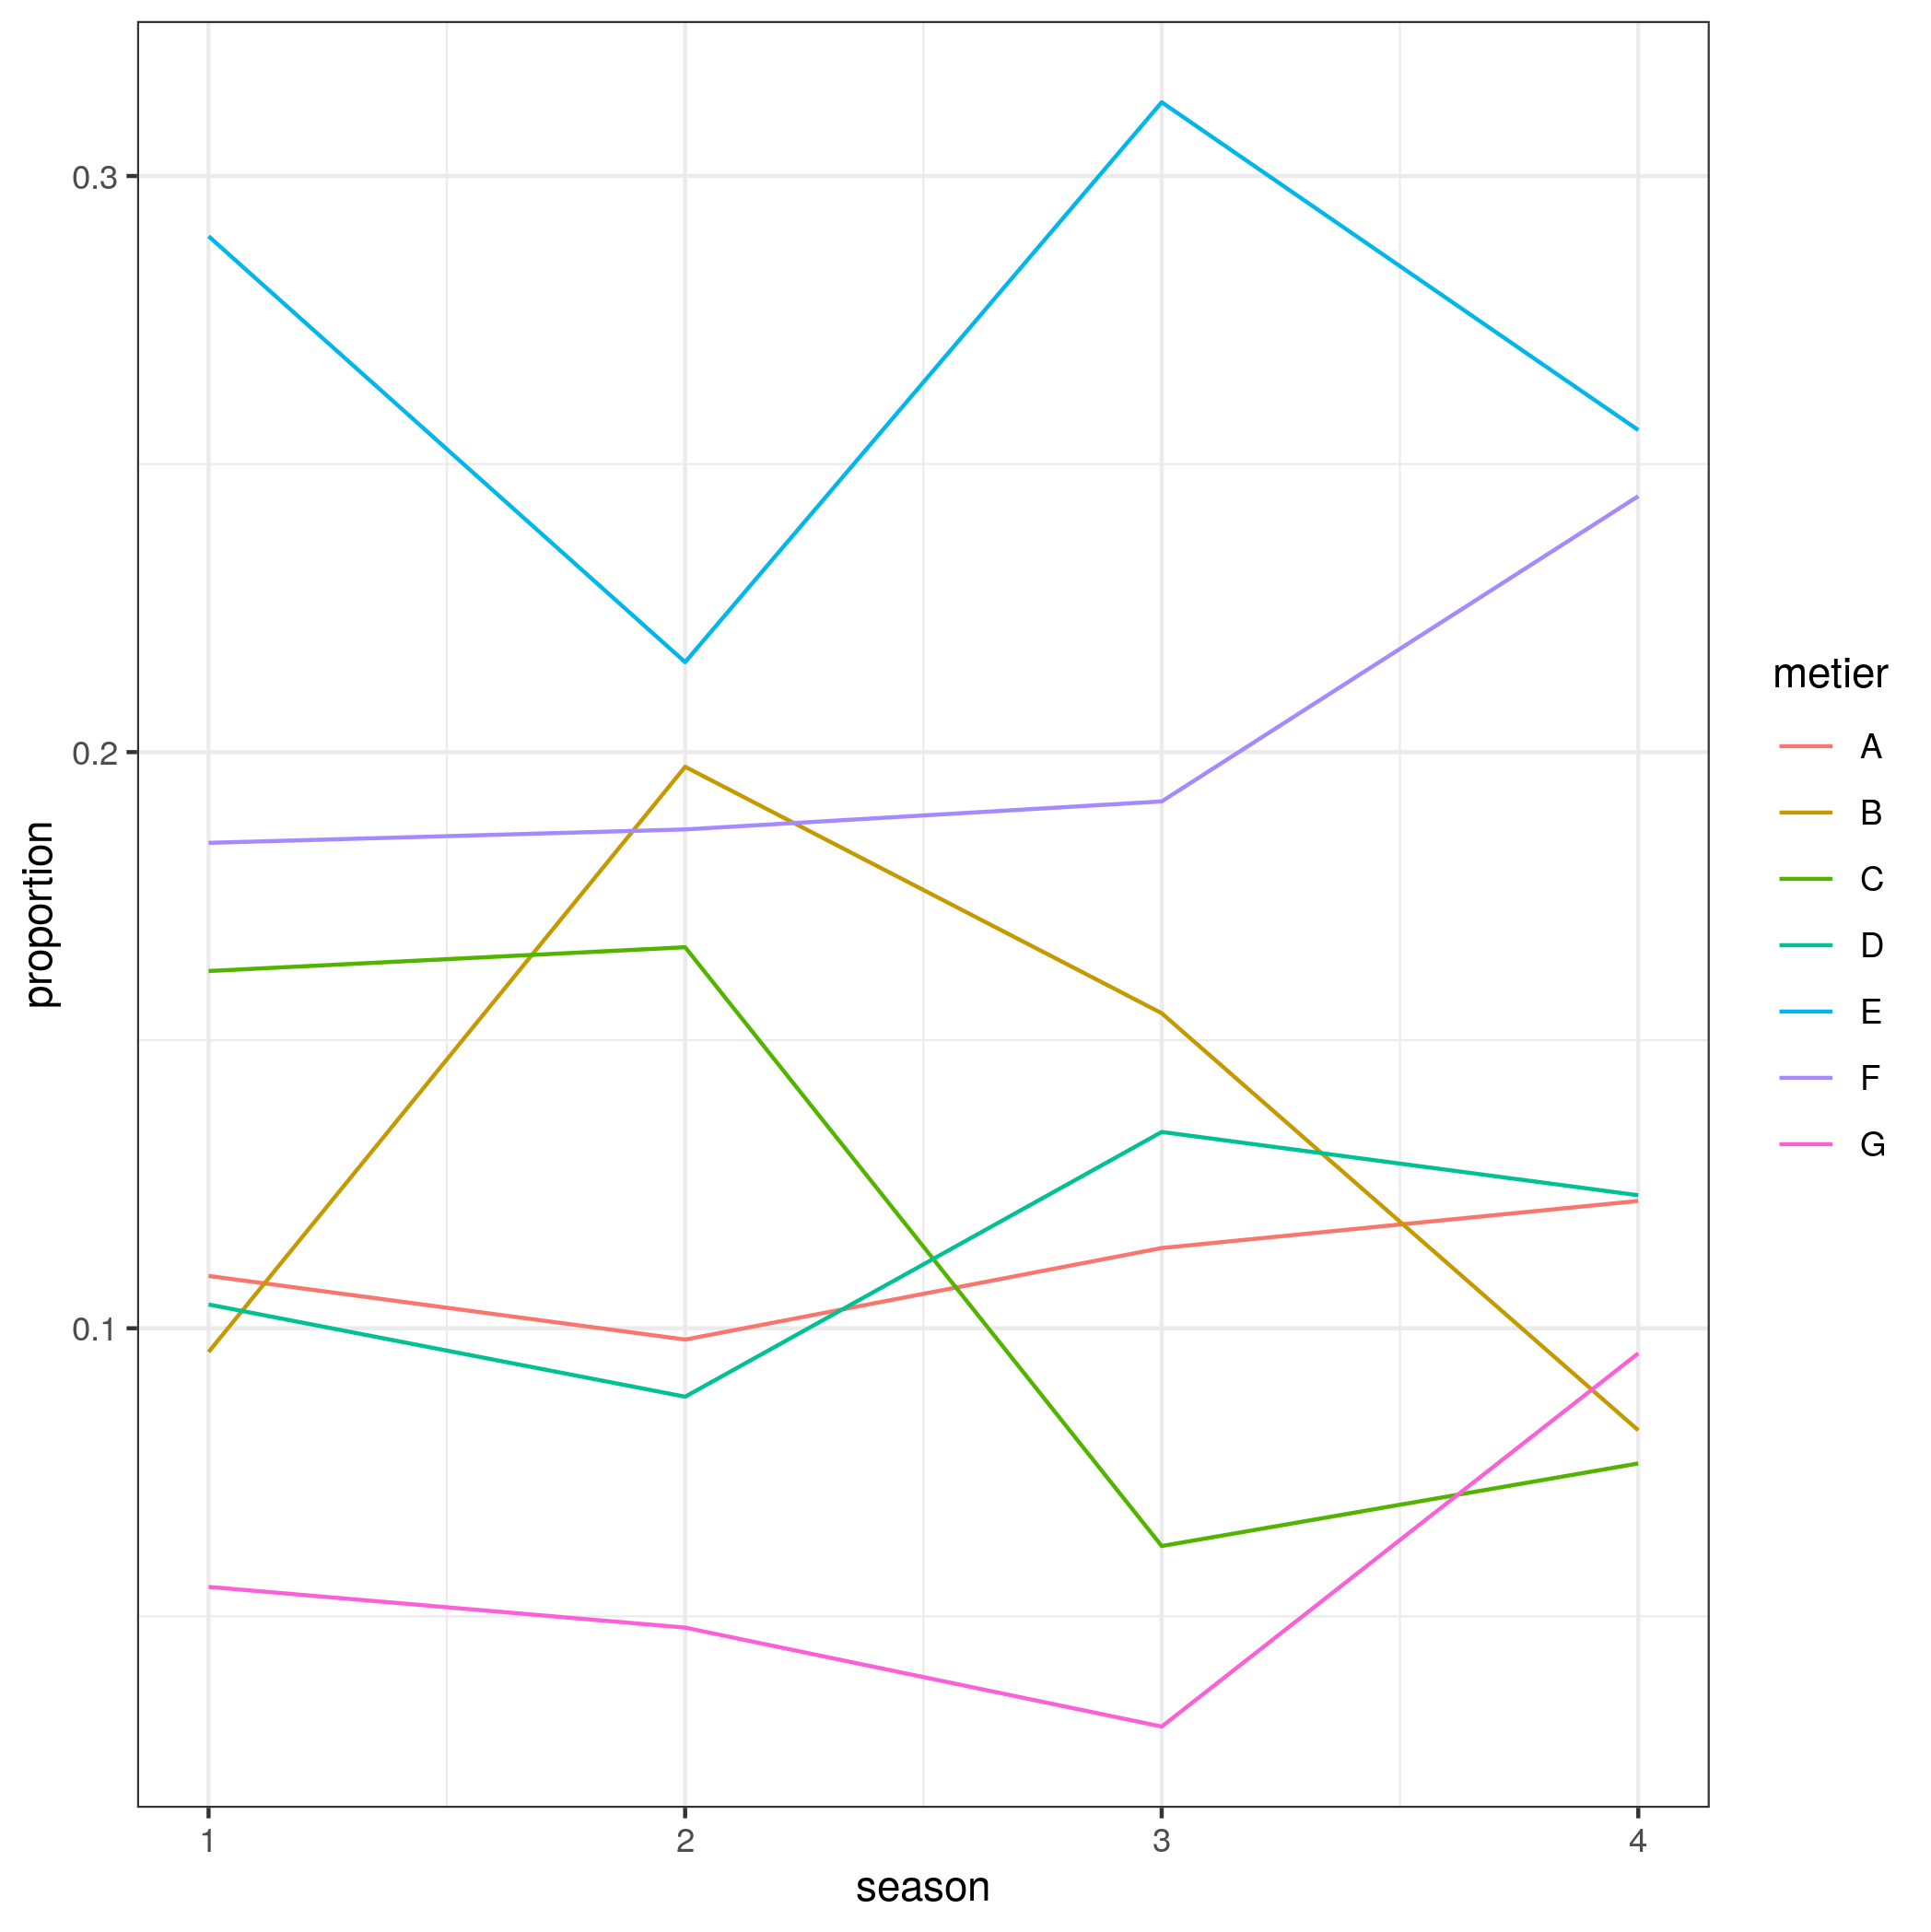
\includegraphics[width=1\linewidth]{figures/Markov_metier_seasonal_effect}
	\caption{Seasonal effect in the Markov model.} 
	\label{fig:Markov_Seas}
\end{figure}	




\begin{figure}[!ht]
	\centering
\begin{subfigure}
	\centering
	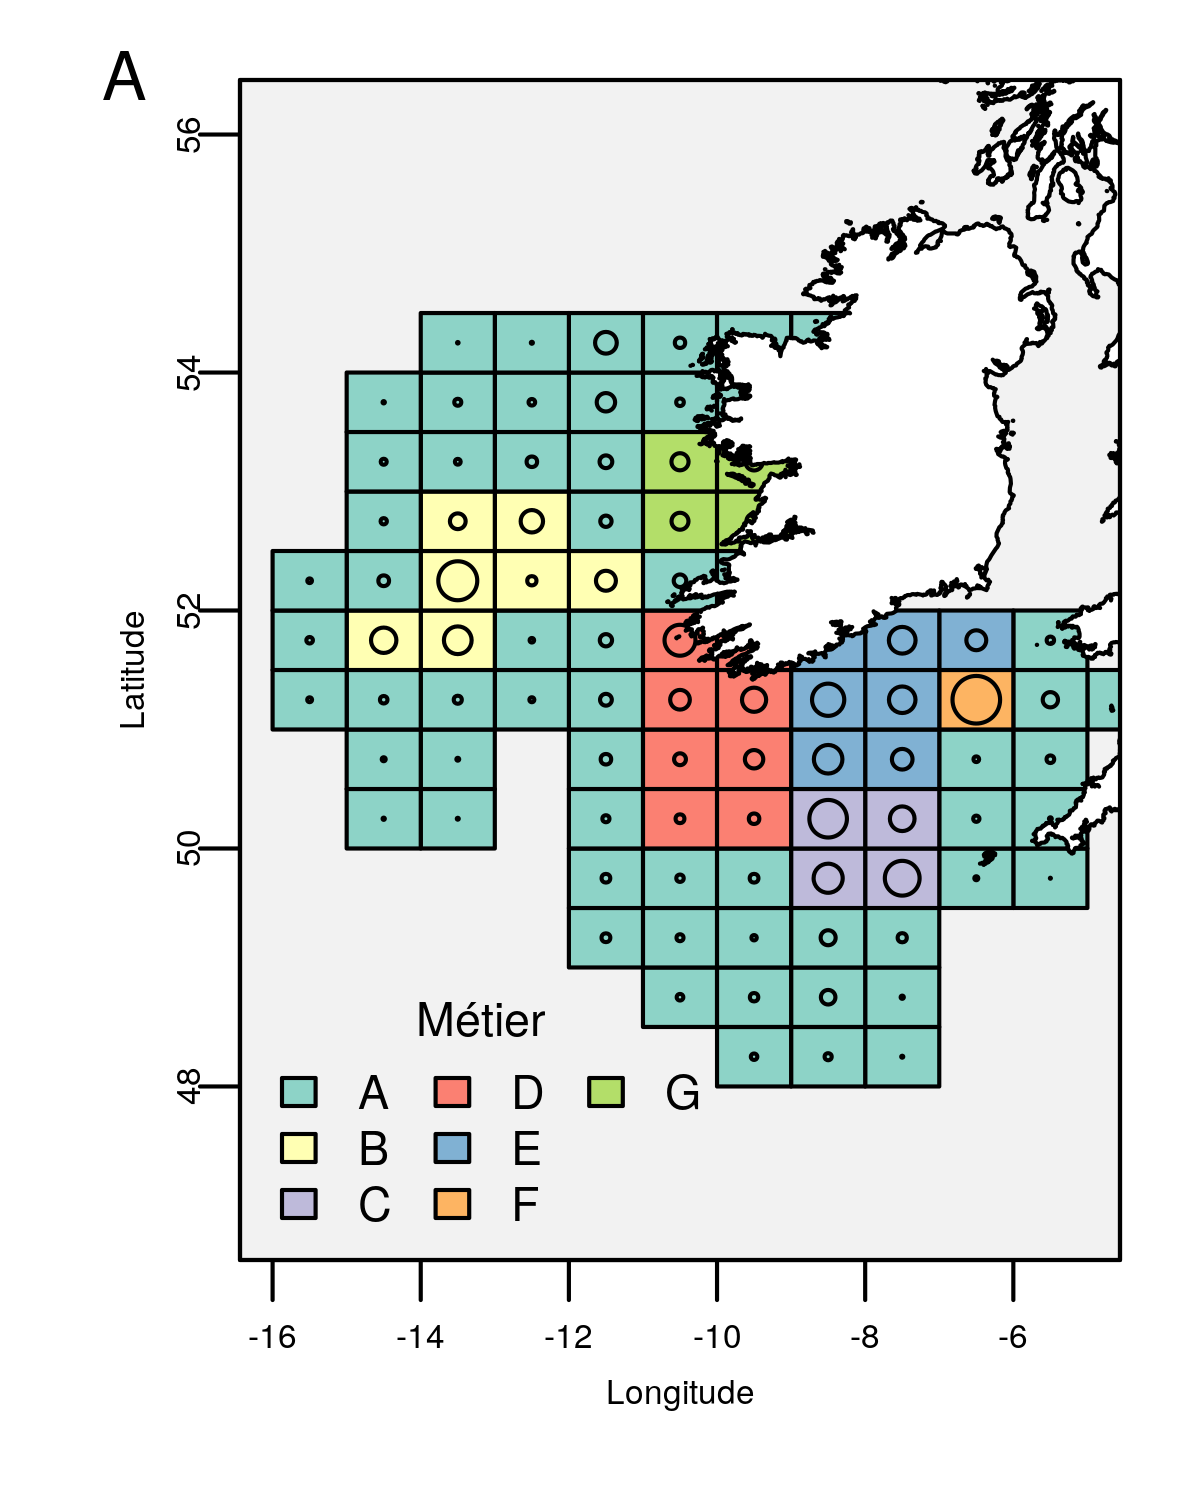
\includegraphics[width=0.8\linewidth]{figures/Final_Metier_locations}
\end{subfigure}
\begin{subfigure}
	\centering
	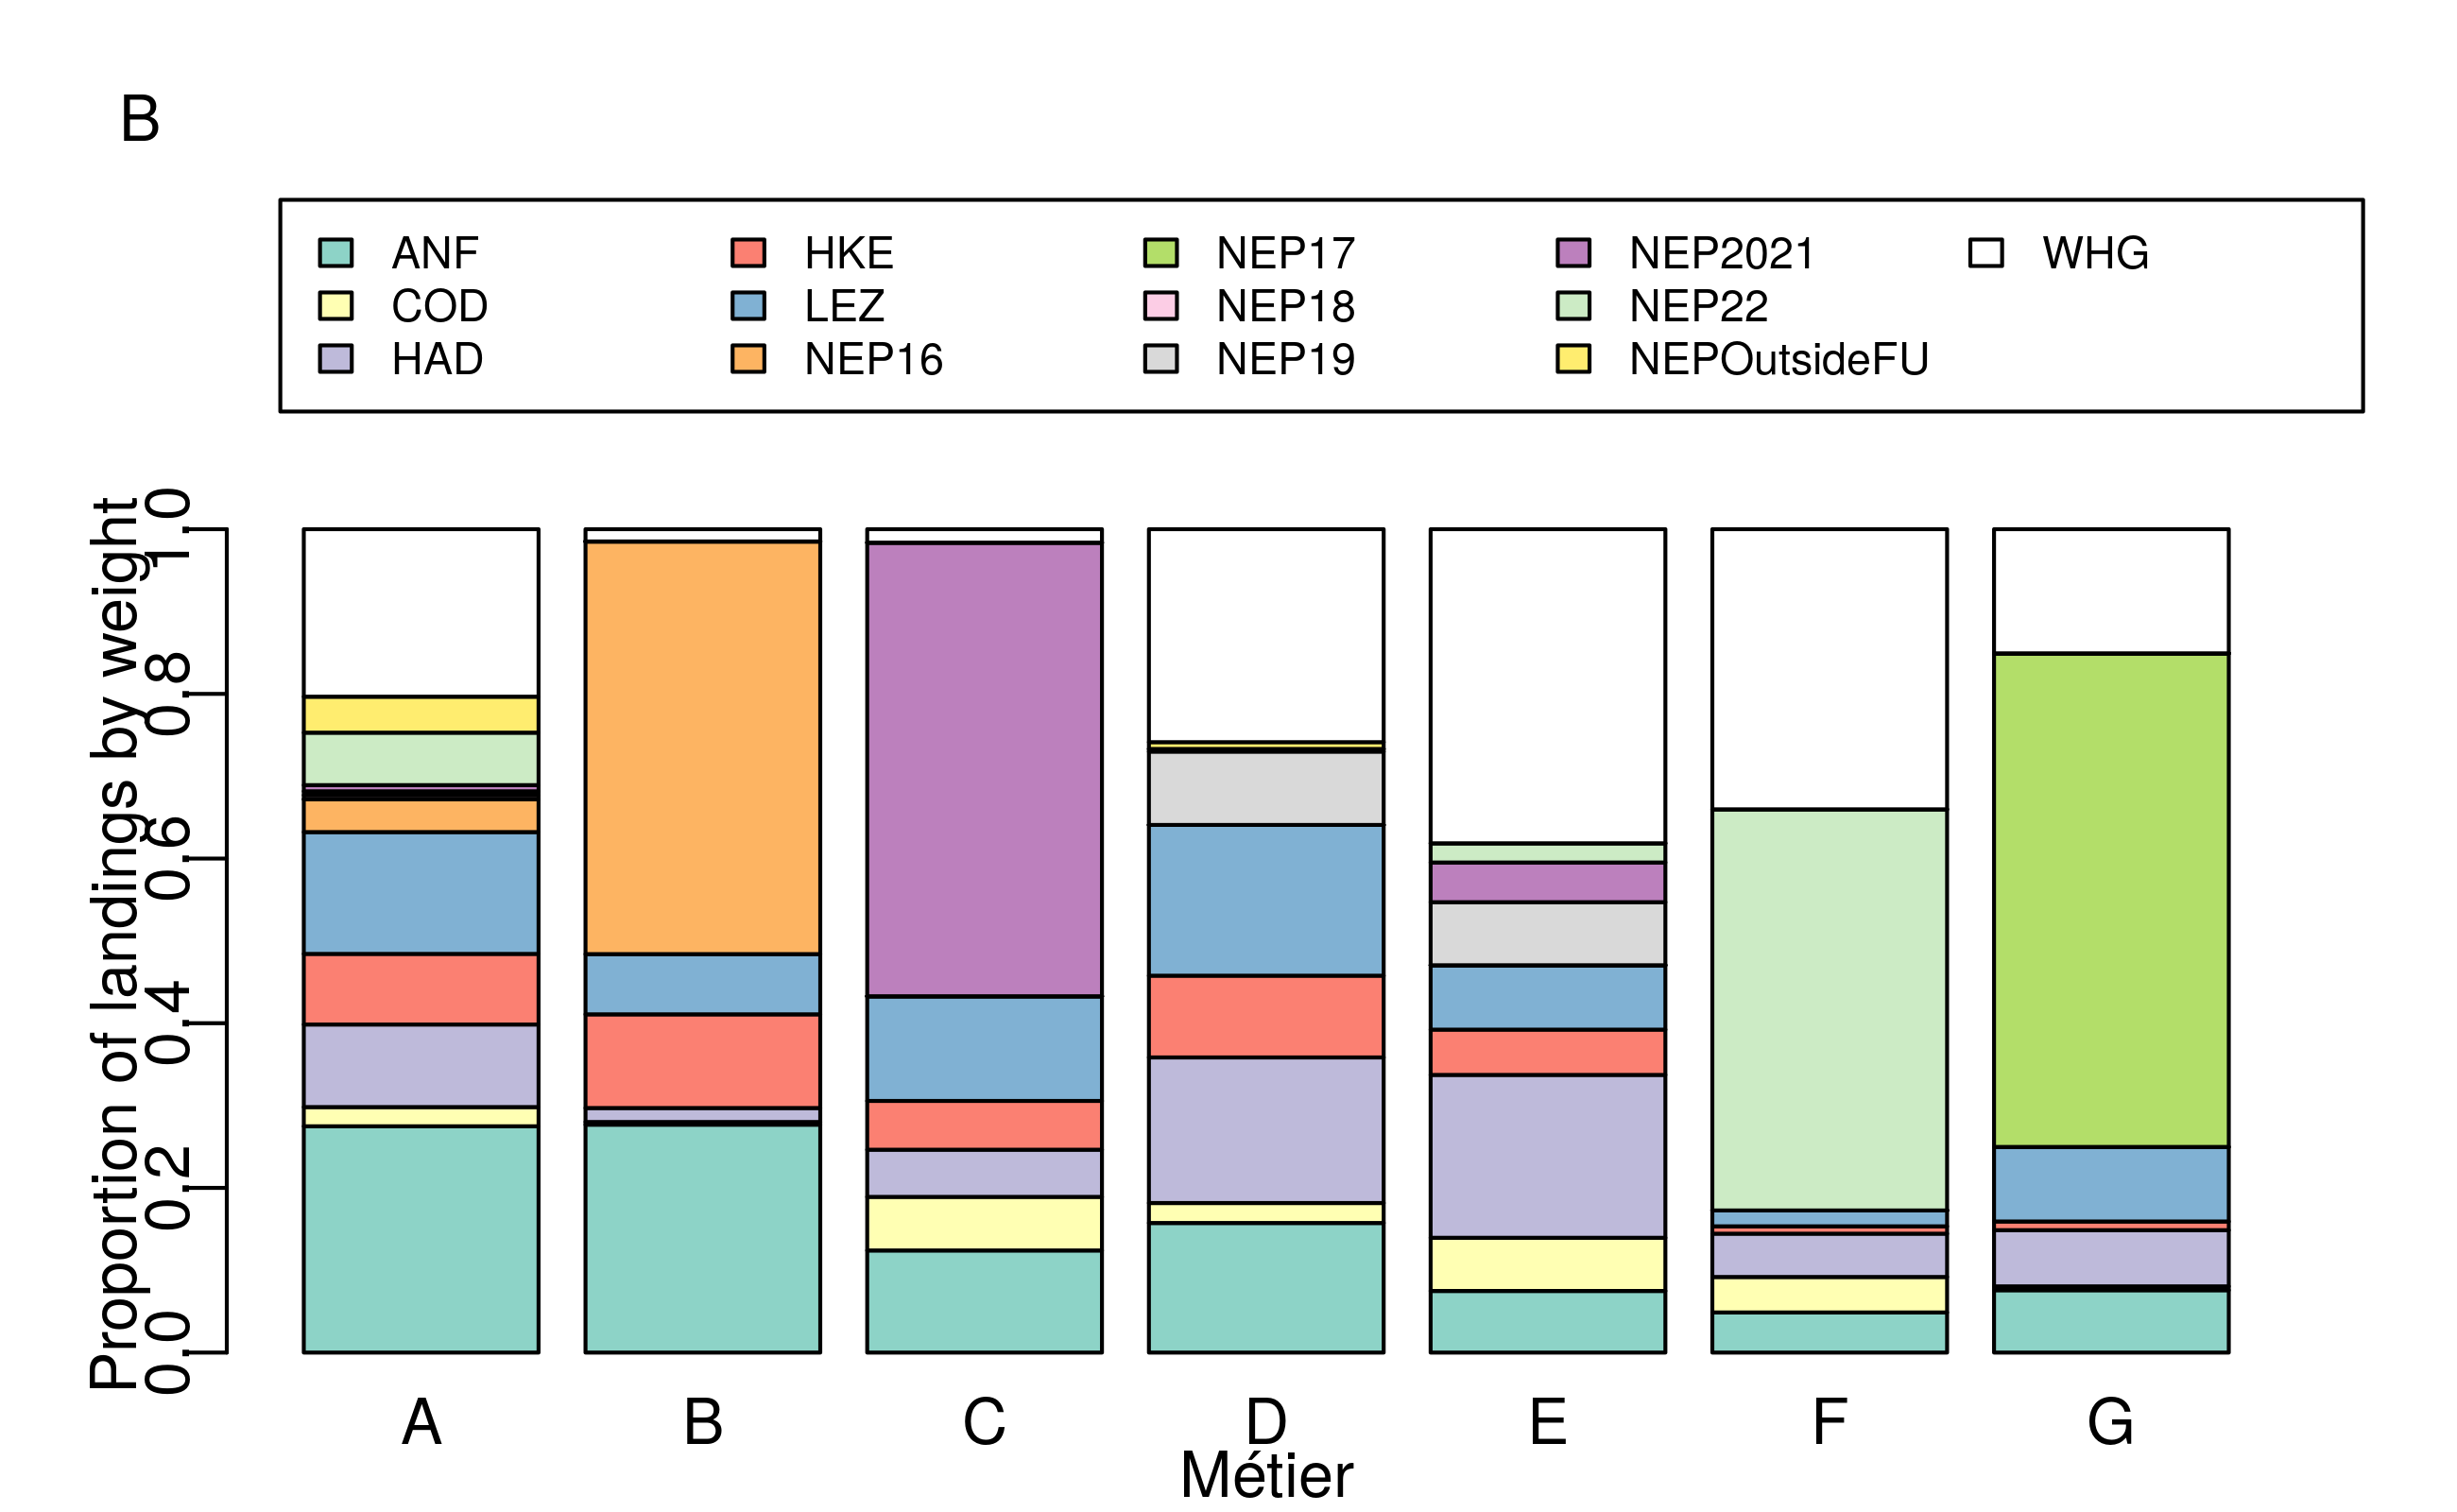
\includegraphics[width=0.8\linewidth]{figures/Final_Metier_catchcomp}
\end{subfigure}
\caption{The métier defined through spatial clustering of similar catch
	composition for Irish Otter trawlers modified by using knowledge of
	fishing grounds to make coherent spatial units. The circles represent
	relative fishing effort in each of the rectangles. Catch compositions
	for the métier indicating the dominant stocks in catches for each of
	the fishing grounds. Stock codes in Table \ref{tab:brp}.} 
	\label{fig:metier}

\end{figure}	

\newpage

\begin{sidewaysfigure}[!ht]
	\centering
	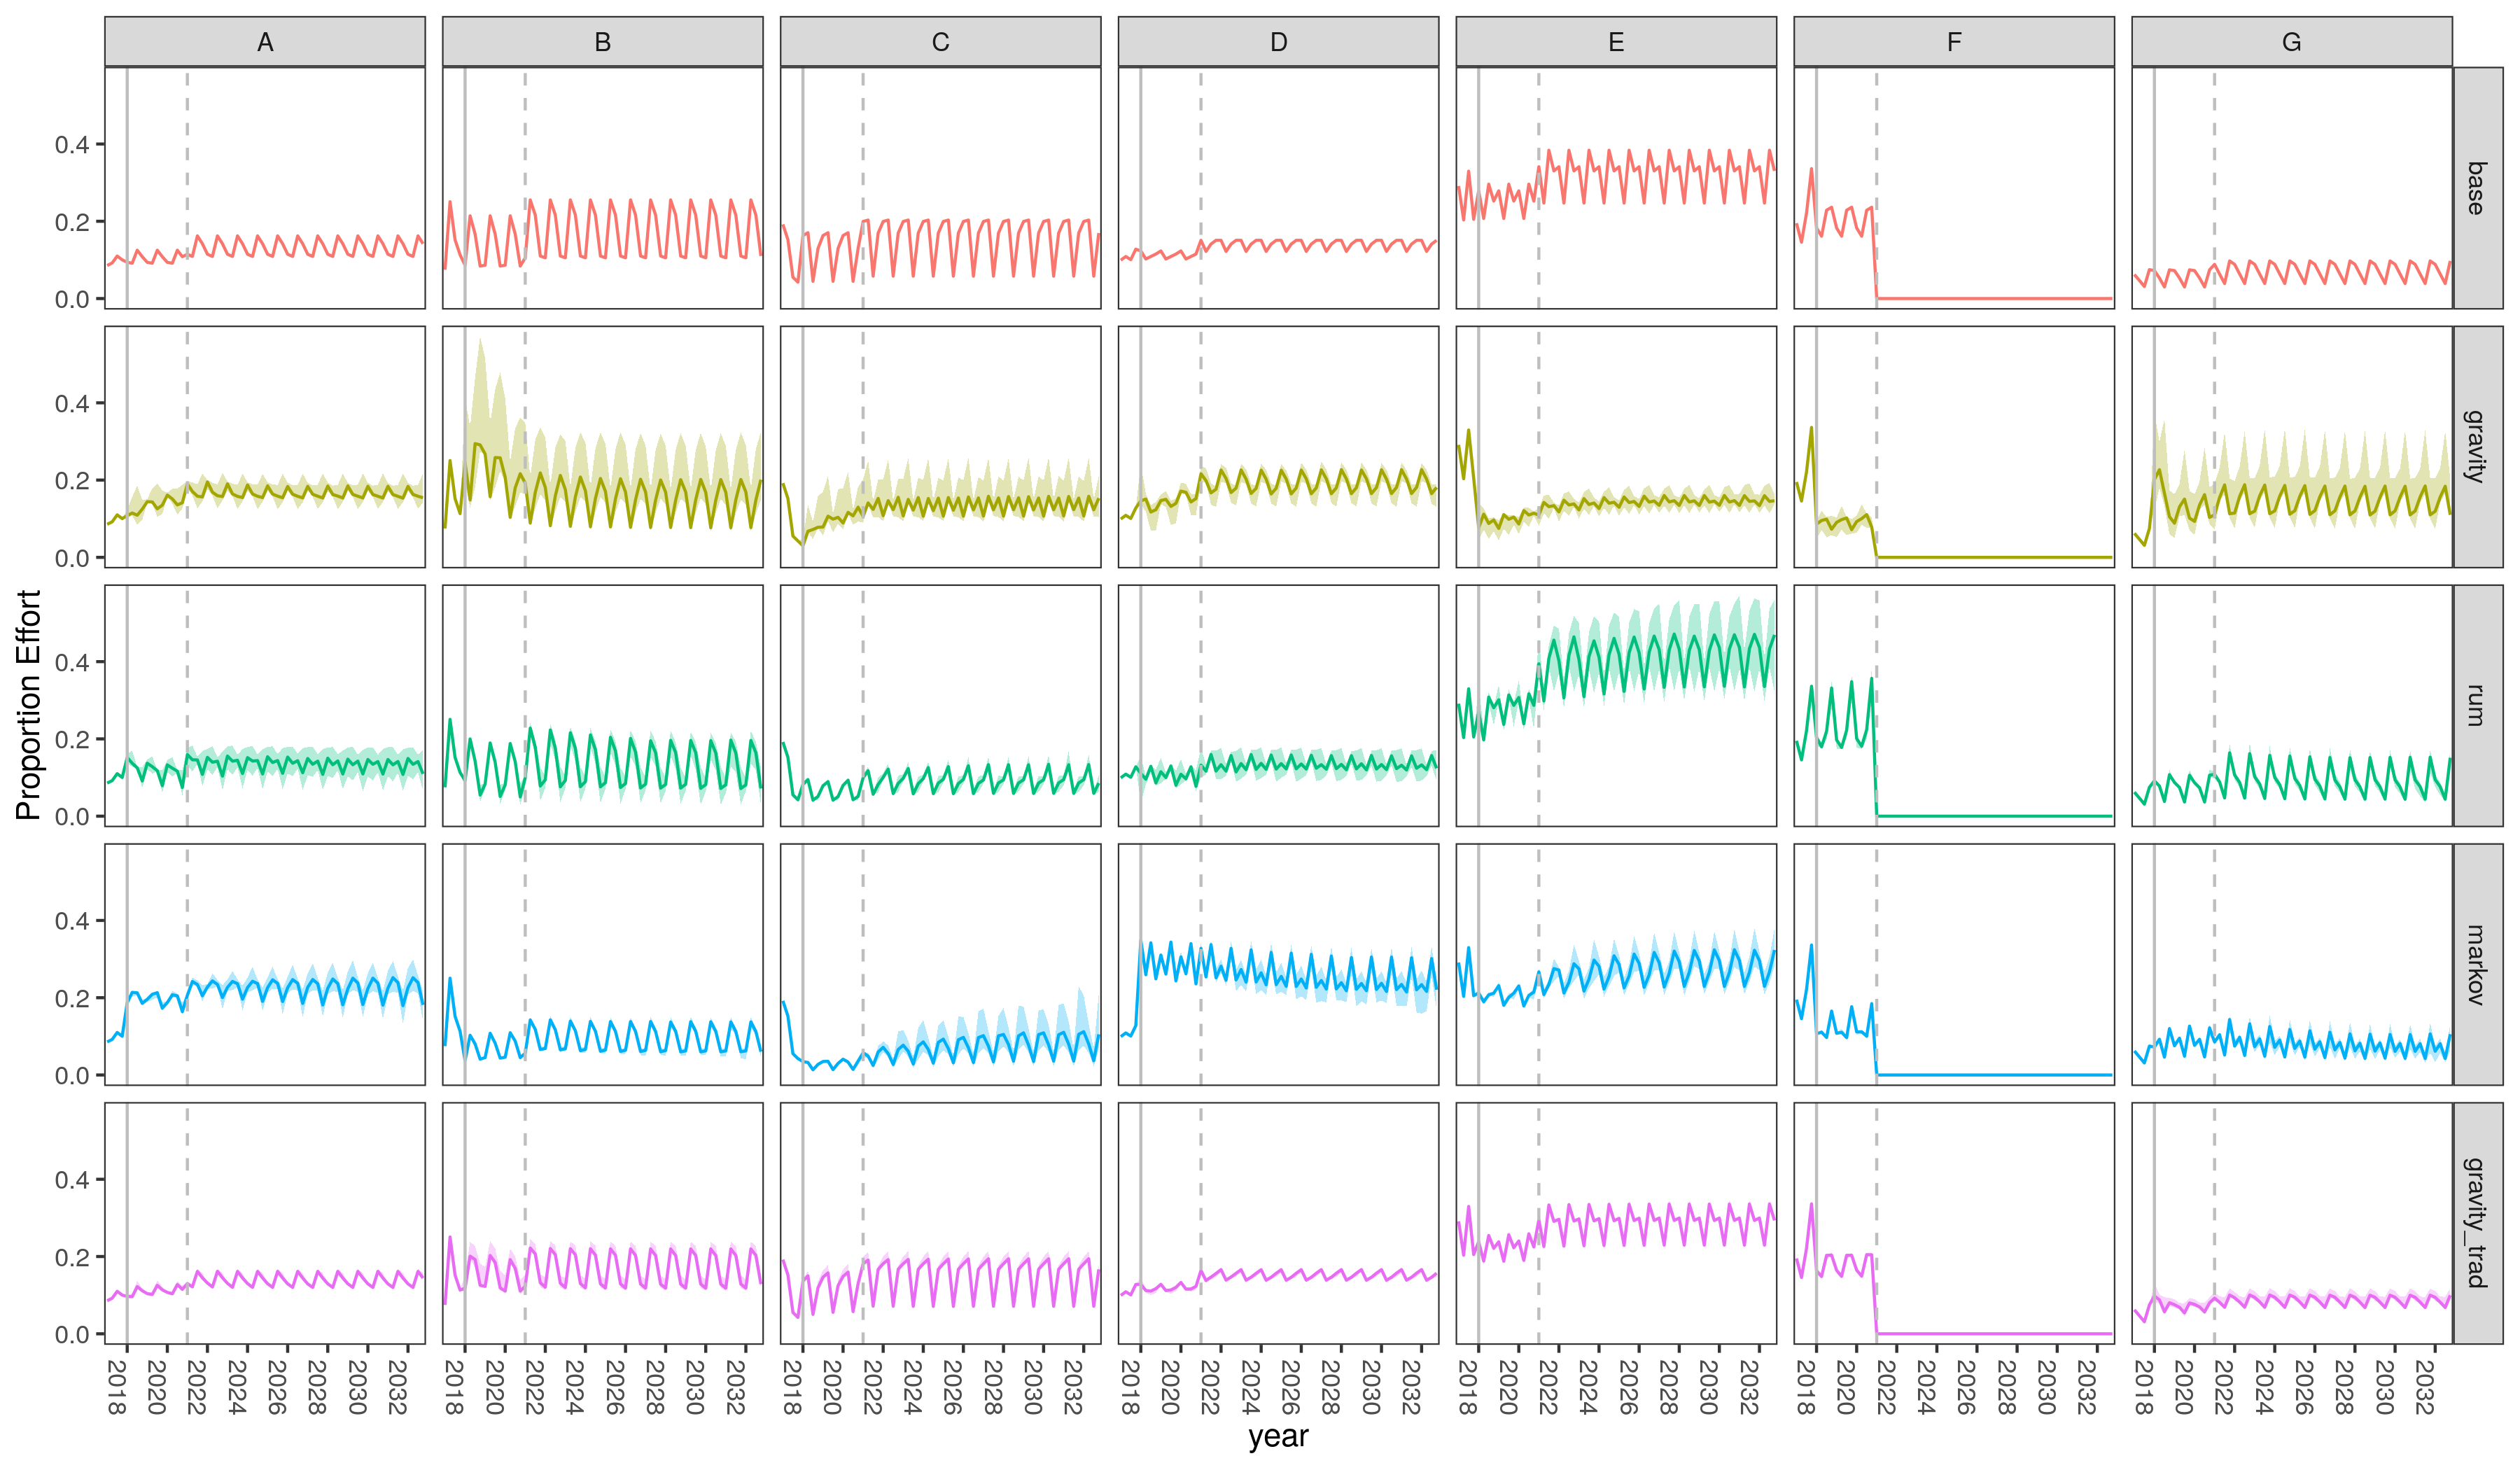
\includegraphics[width=1\linewidth]{figures/Effort_shares}
	\caption{Quarterly fishing effort share (proportion) for each métier
		and location choice model (2017 - 2032). Light shading
		represents 5\% and 95\% variability due to recruitment and
		catchability. Solid line indicates end of the data/start of
		simulations and the dashed line the implementation of the
		spatial closure.} 
	\label{fig:effort}
\end{sidewaysfigure}	

\newpage

\begin{figure}[!ht]
	\centering
	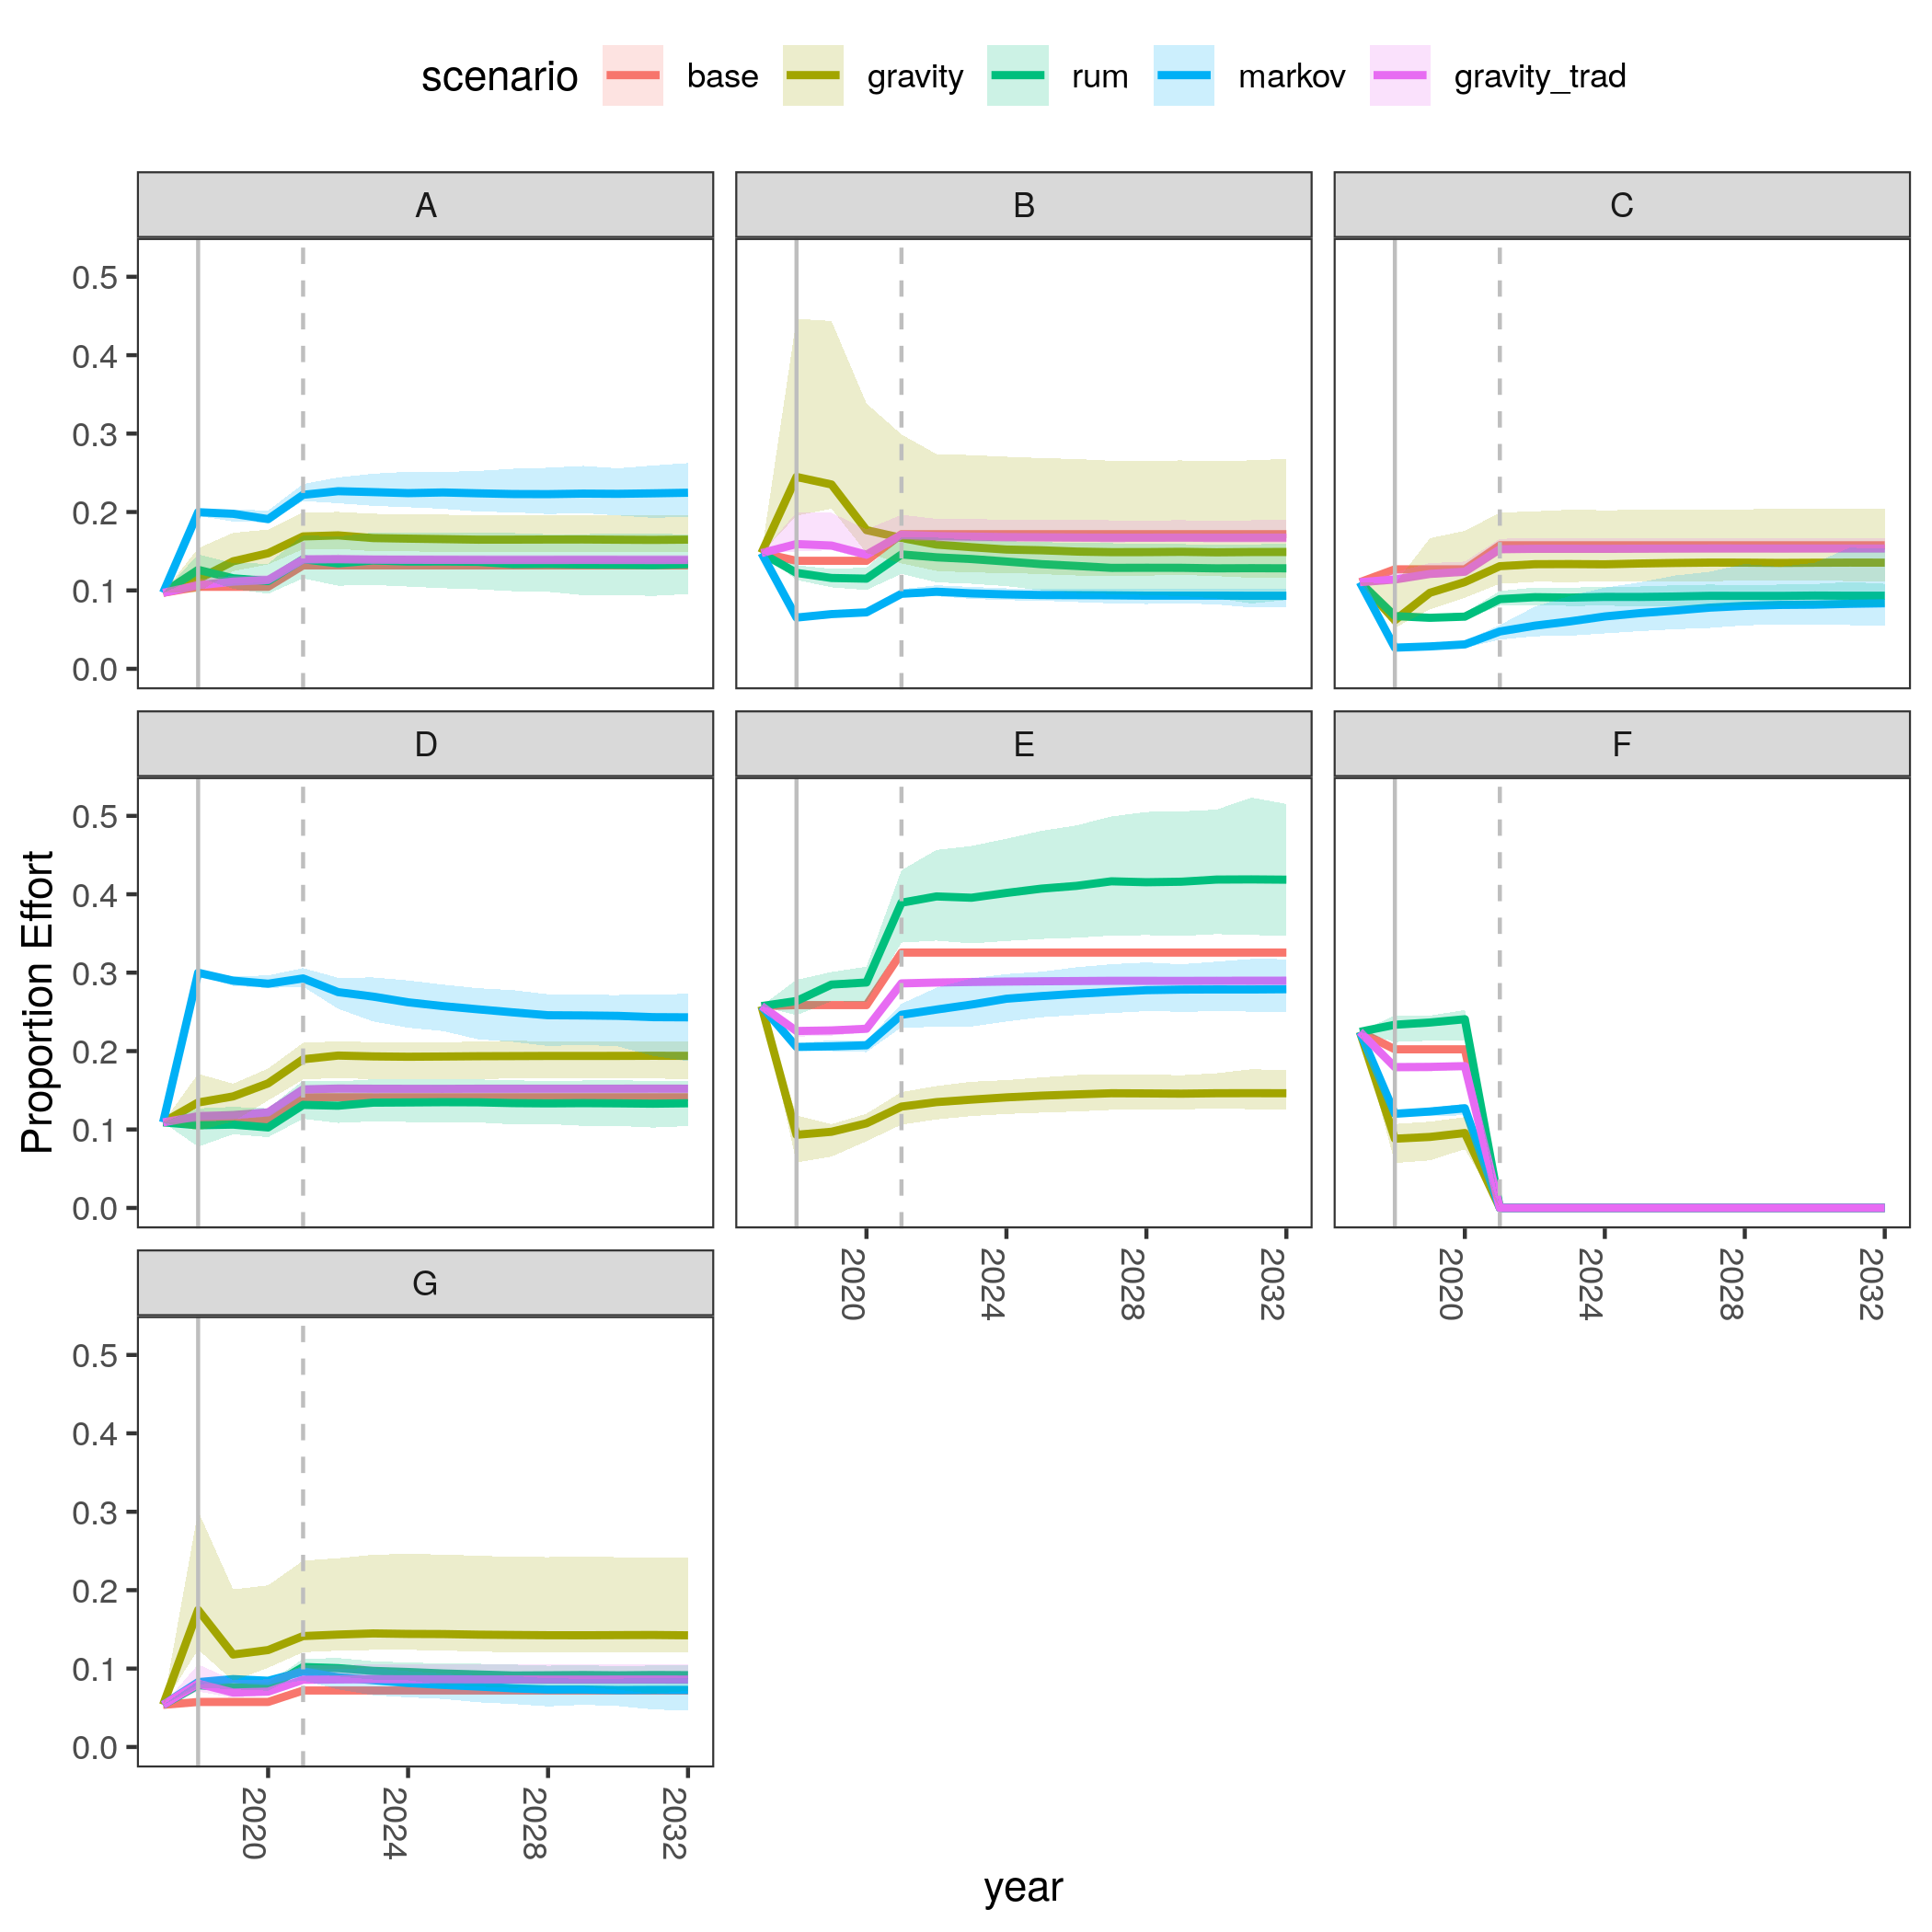
\includegraphics[width=1\linewidth]{figures/Effort_shares_annual}
	\caption{Annualised effort share (proportion) for each métier
		and location choice model (2017 - 2032). Light shading
		represents 5\% and 95\% variability due to recruitment and
		catchability. Solid line indicates end of the data/start of
		simulations and the dashed line the implementation of the
		spatial closure.} 
	\label{fig:effort_an}
\end{figure}	

\begin{figure}[!ht]
	\centering
	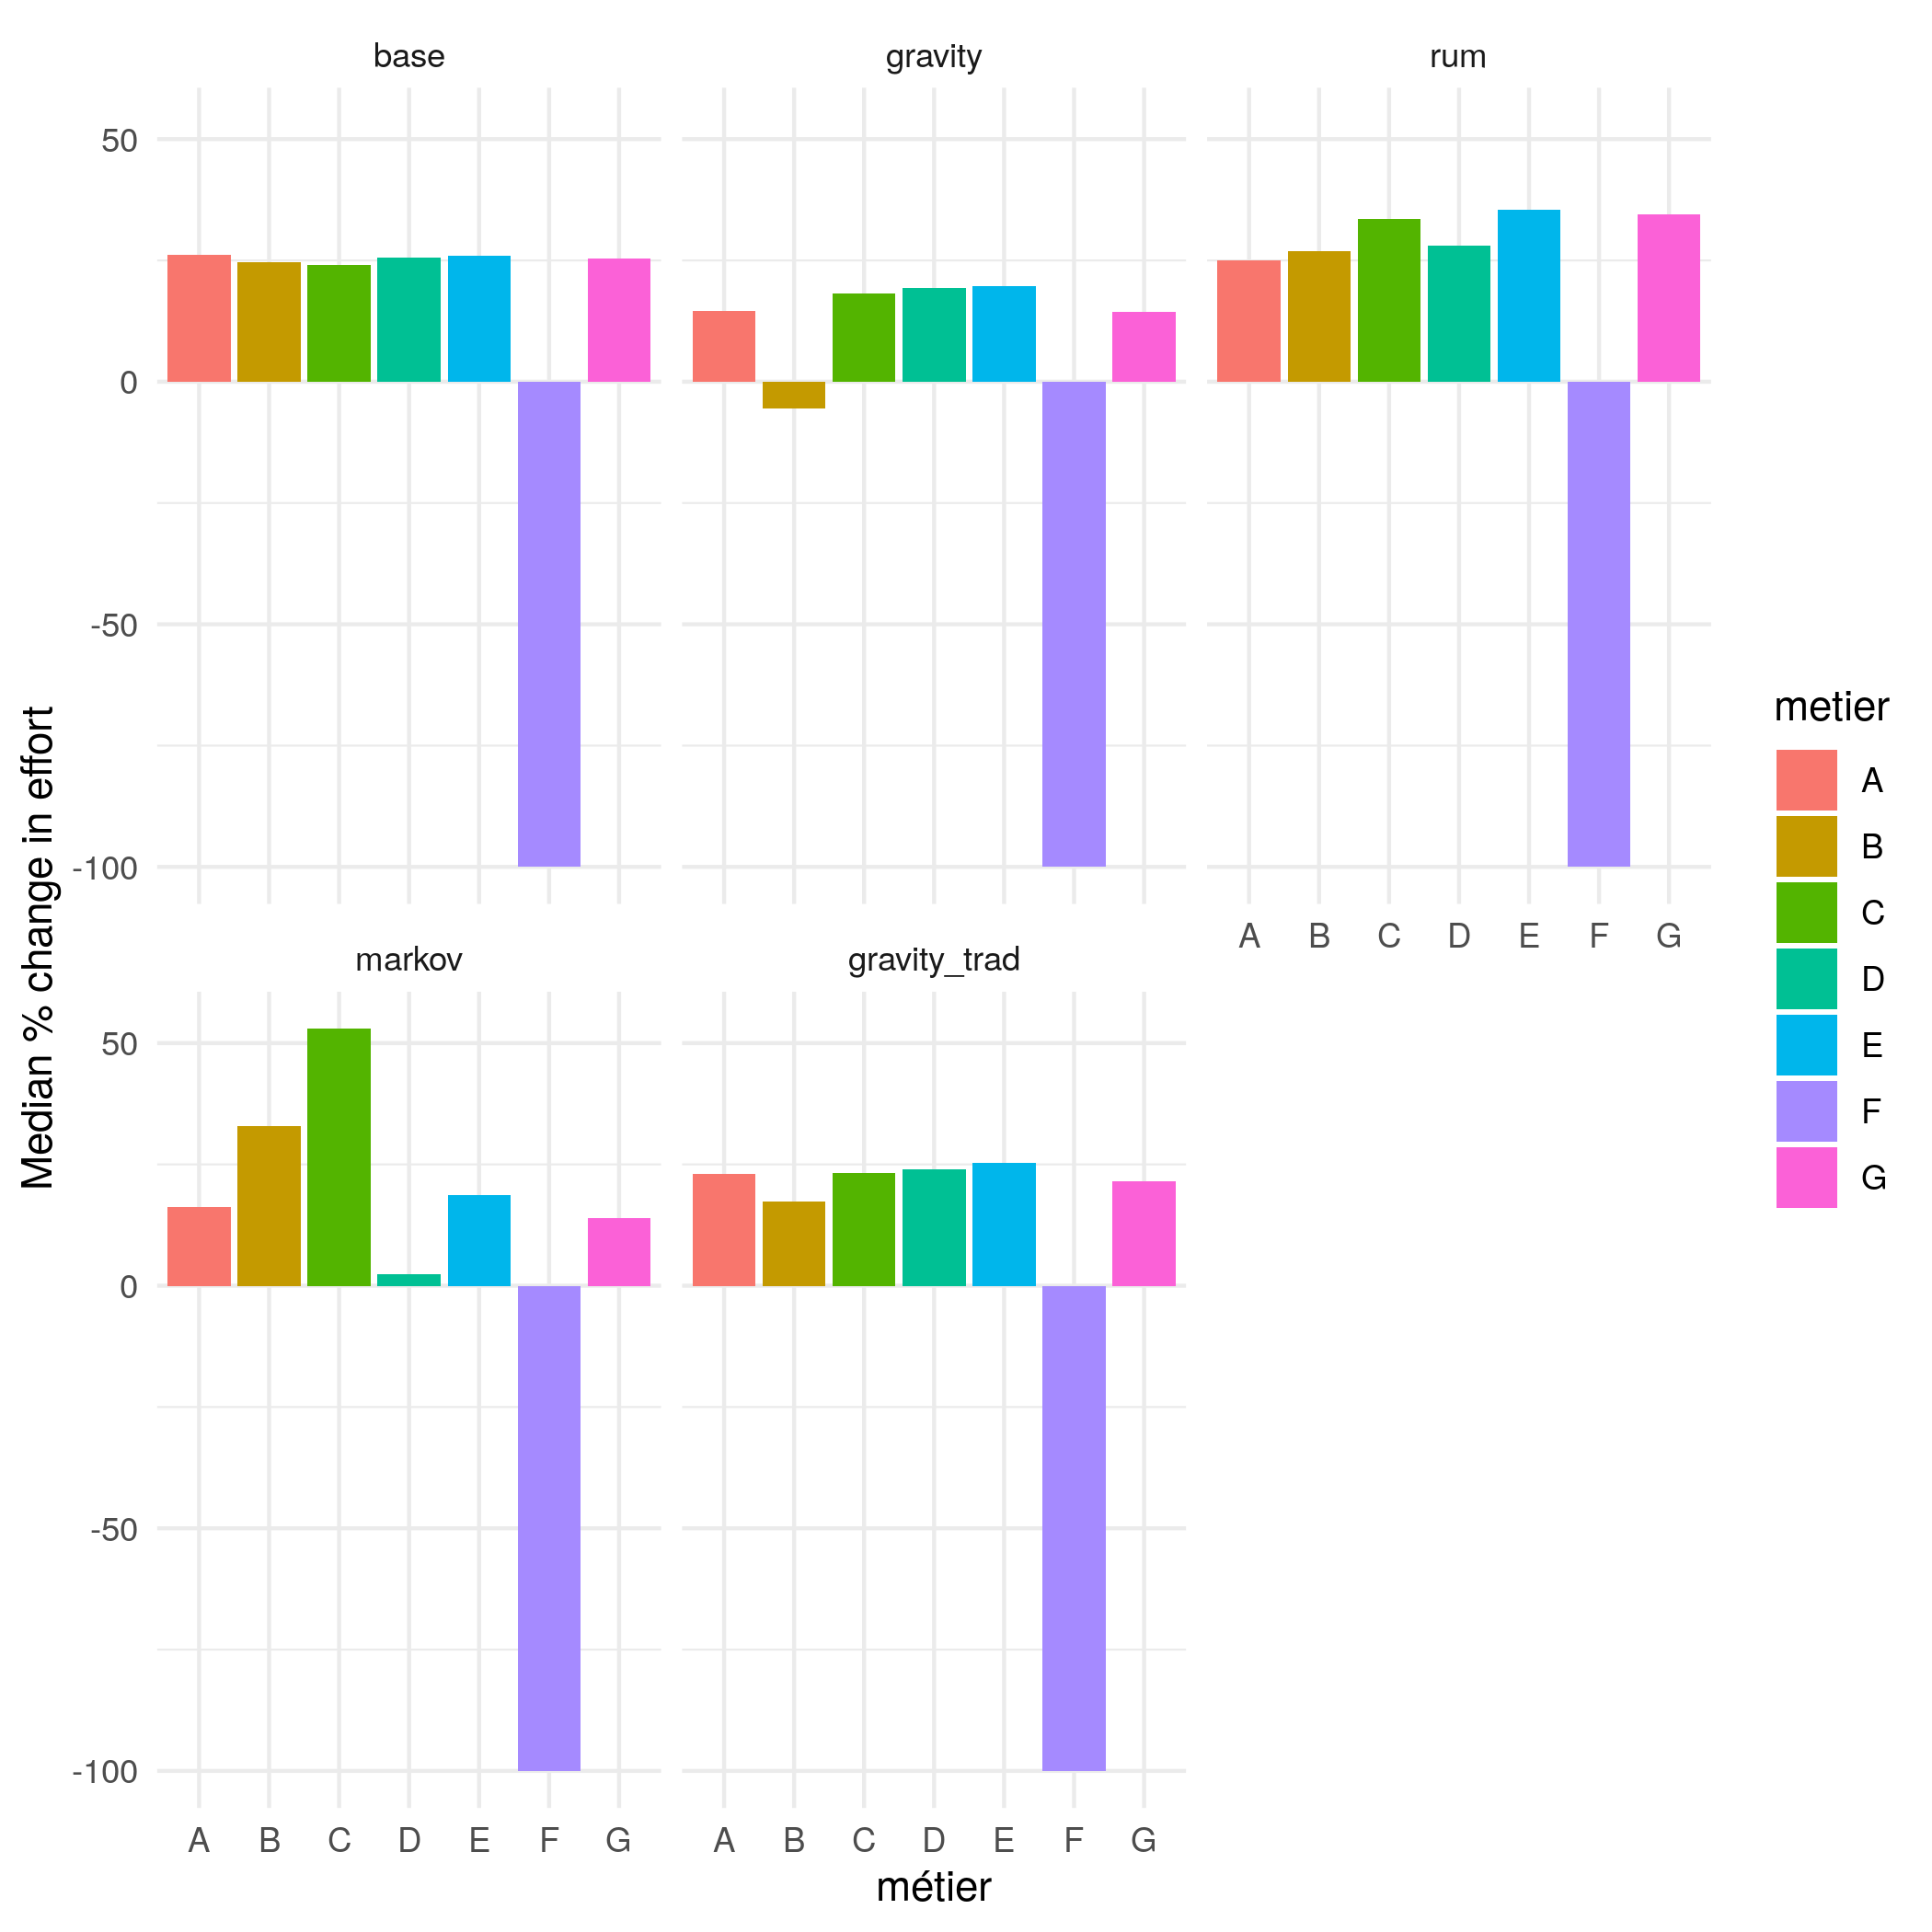
\includegraphics[width=1\linewidth]{figures/Change_effort}
	\caption{Percentage change in annualised effort share for each of the
		métier from before (2020) the closure of métier F and first
		year of the closure (2021).} 
	\label{fig:effort_chg}
\end{figure}	



\begin{figure}[!ht]
	\centering
	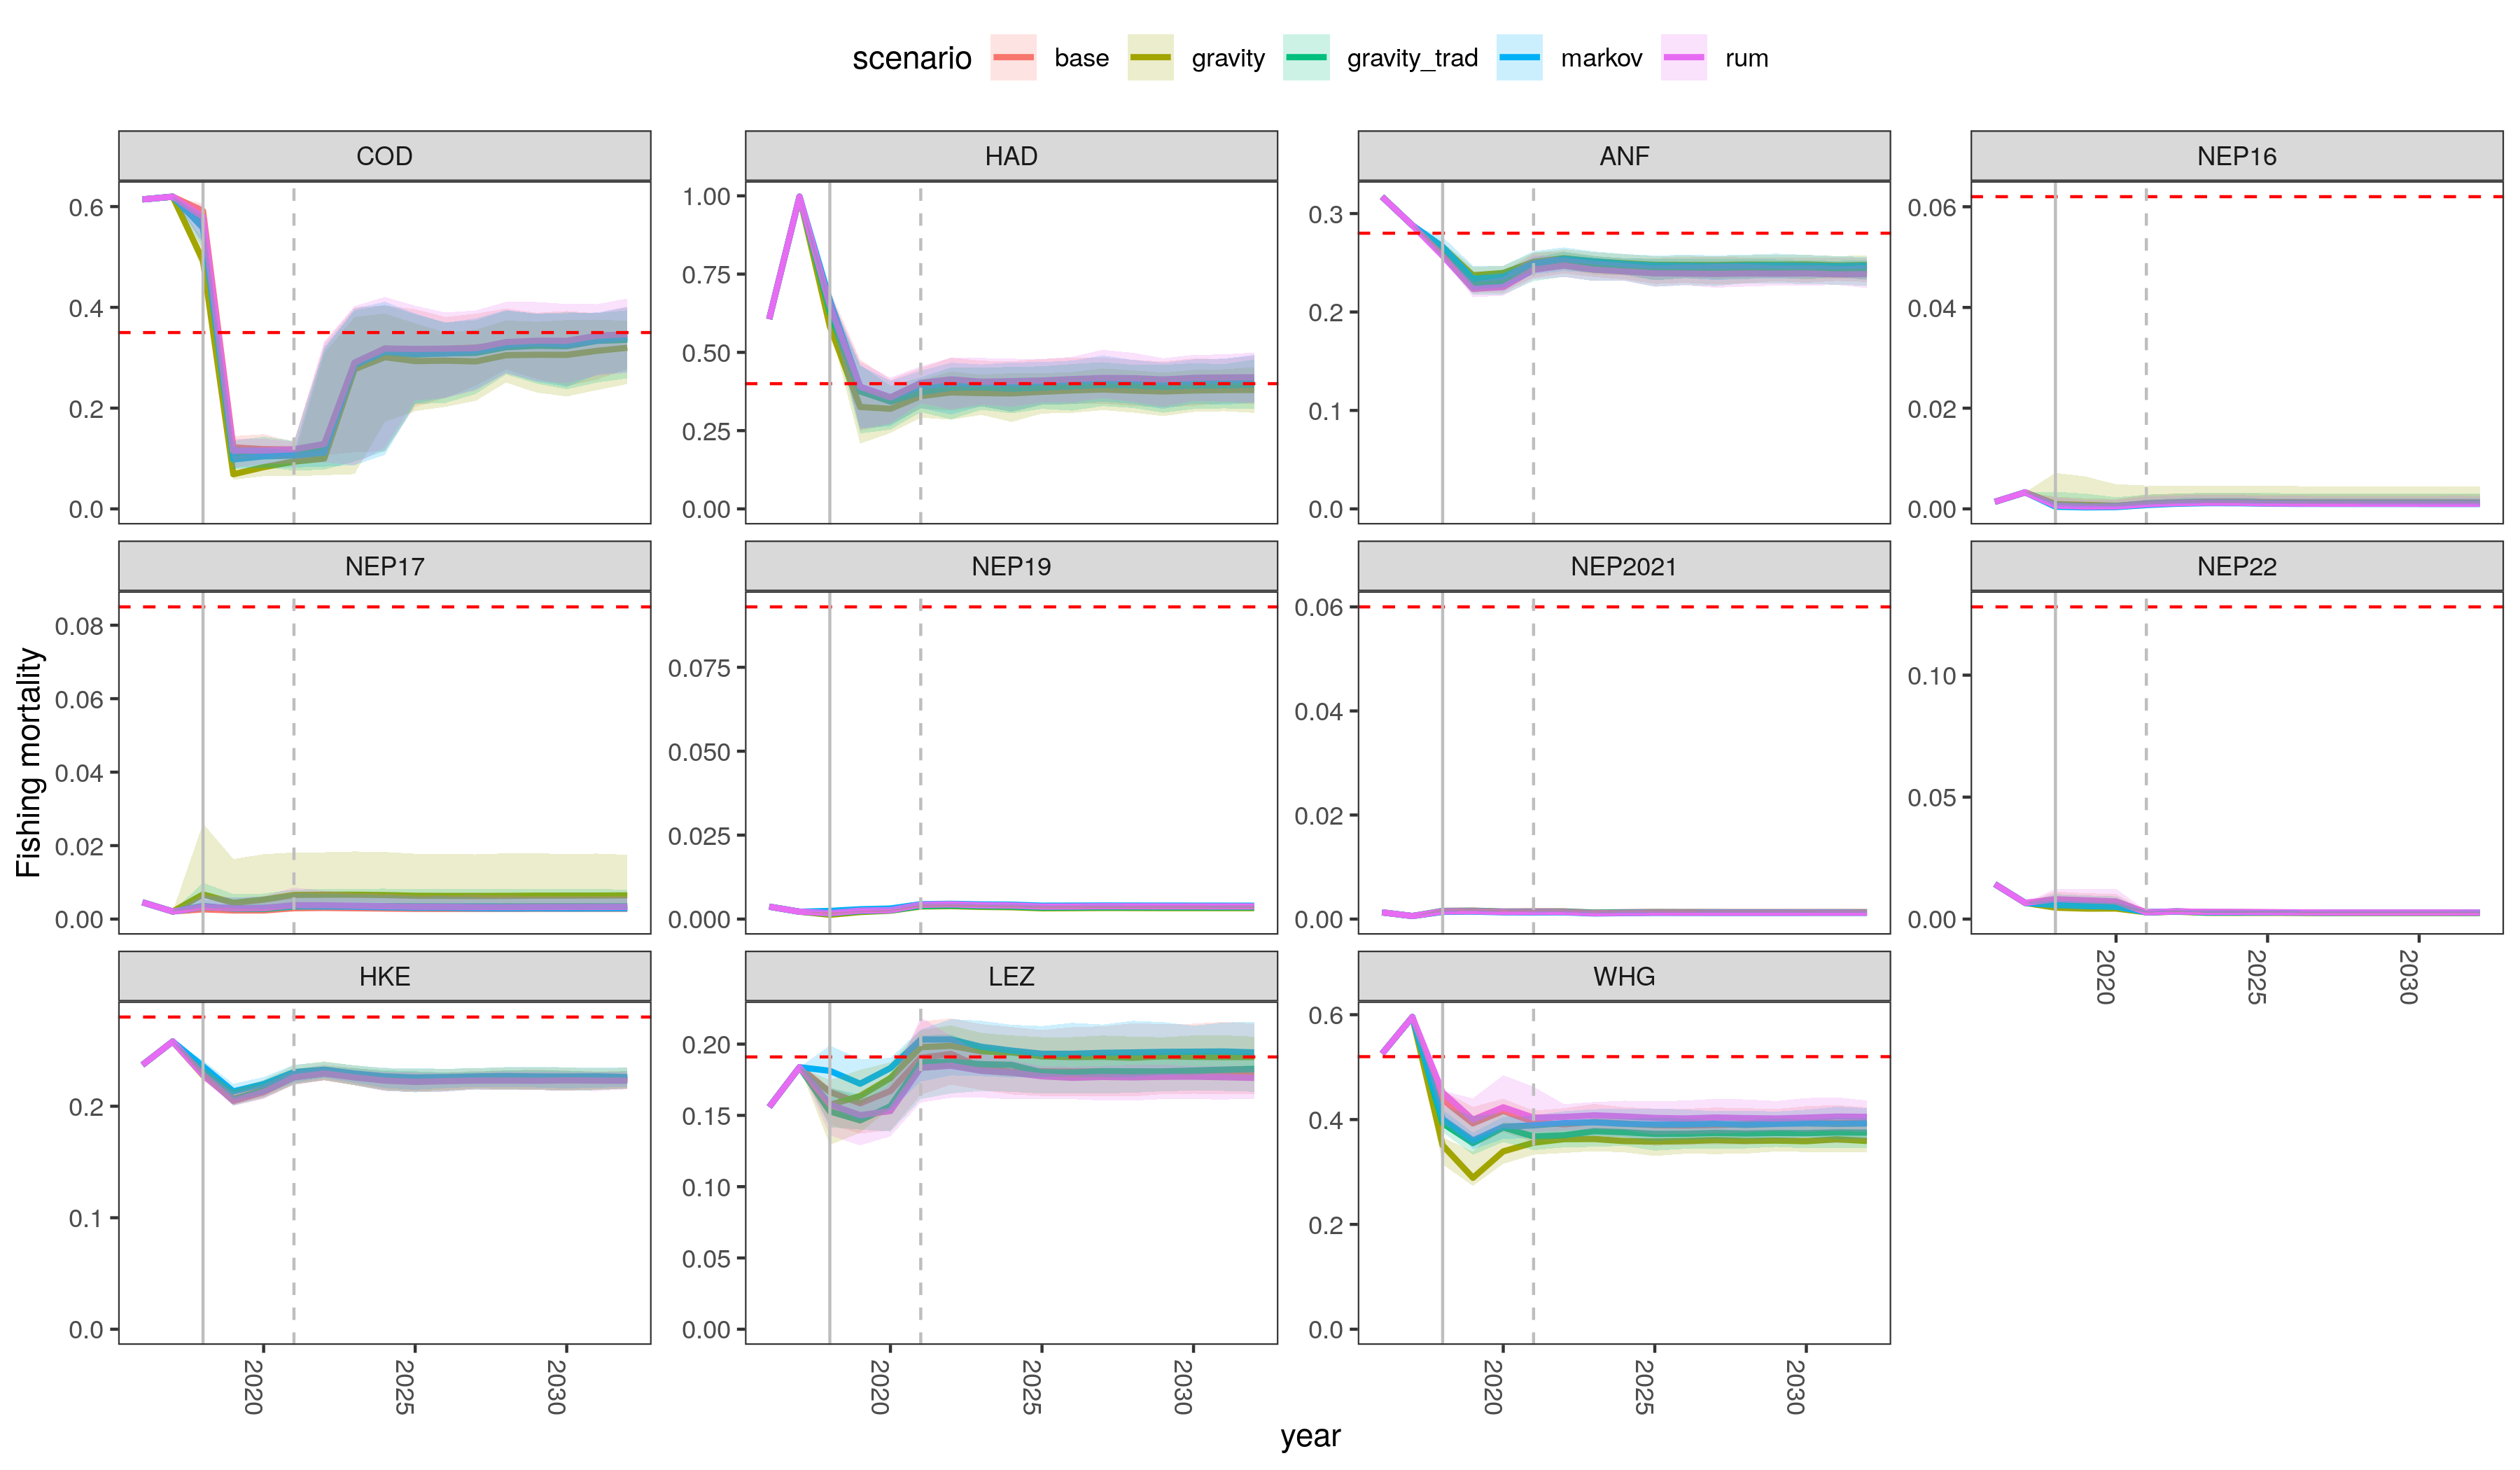
\includegraphics[width=1\linewidth]{figures/F_difference}
	\caption{Fishing mortality for each stock under the different location
		choice models. Each stock was targeted to be fished at its Fmsy
		rate, using the ICES MSY Harvest Control Rule. Light shading
		represents 5\% and 95\% variability due to recruitment and
		catchability. Solid line indicates end of the data/start of
		simulations and the dashed line the implementation of the
		spatial closure. Dashed red lines indicate the stock Fmsy
		reference point.} 
	\label{fig:F}
\end{figure}	

\begin{figure}[!ht]
	\centering
	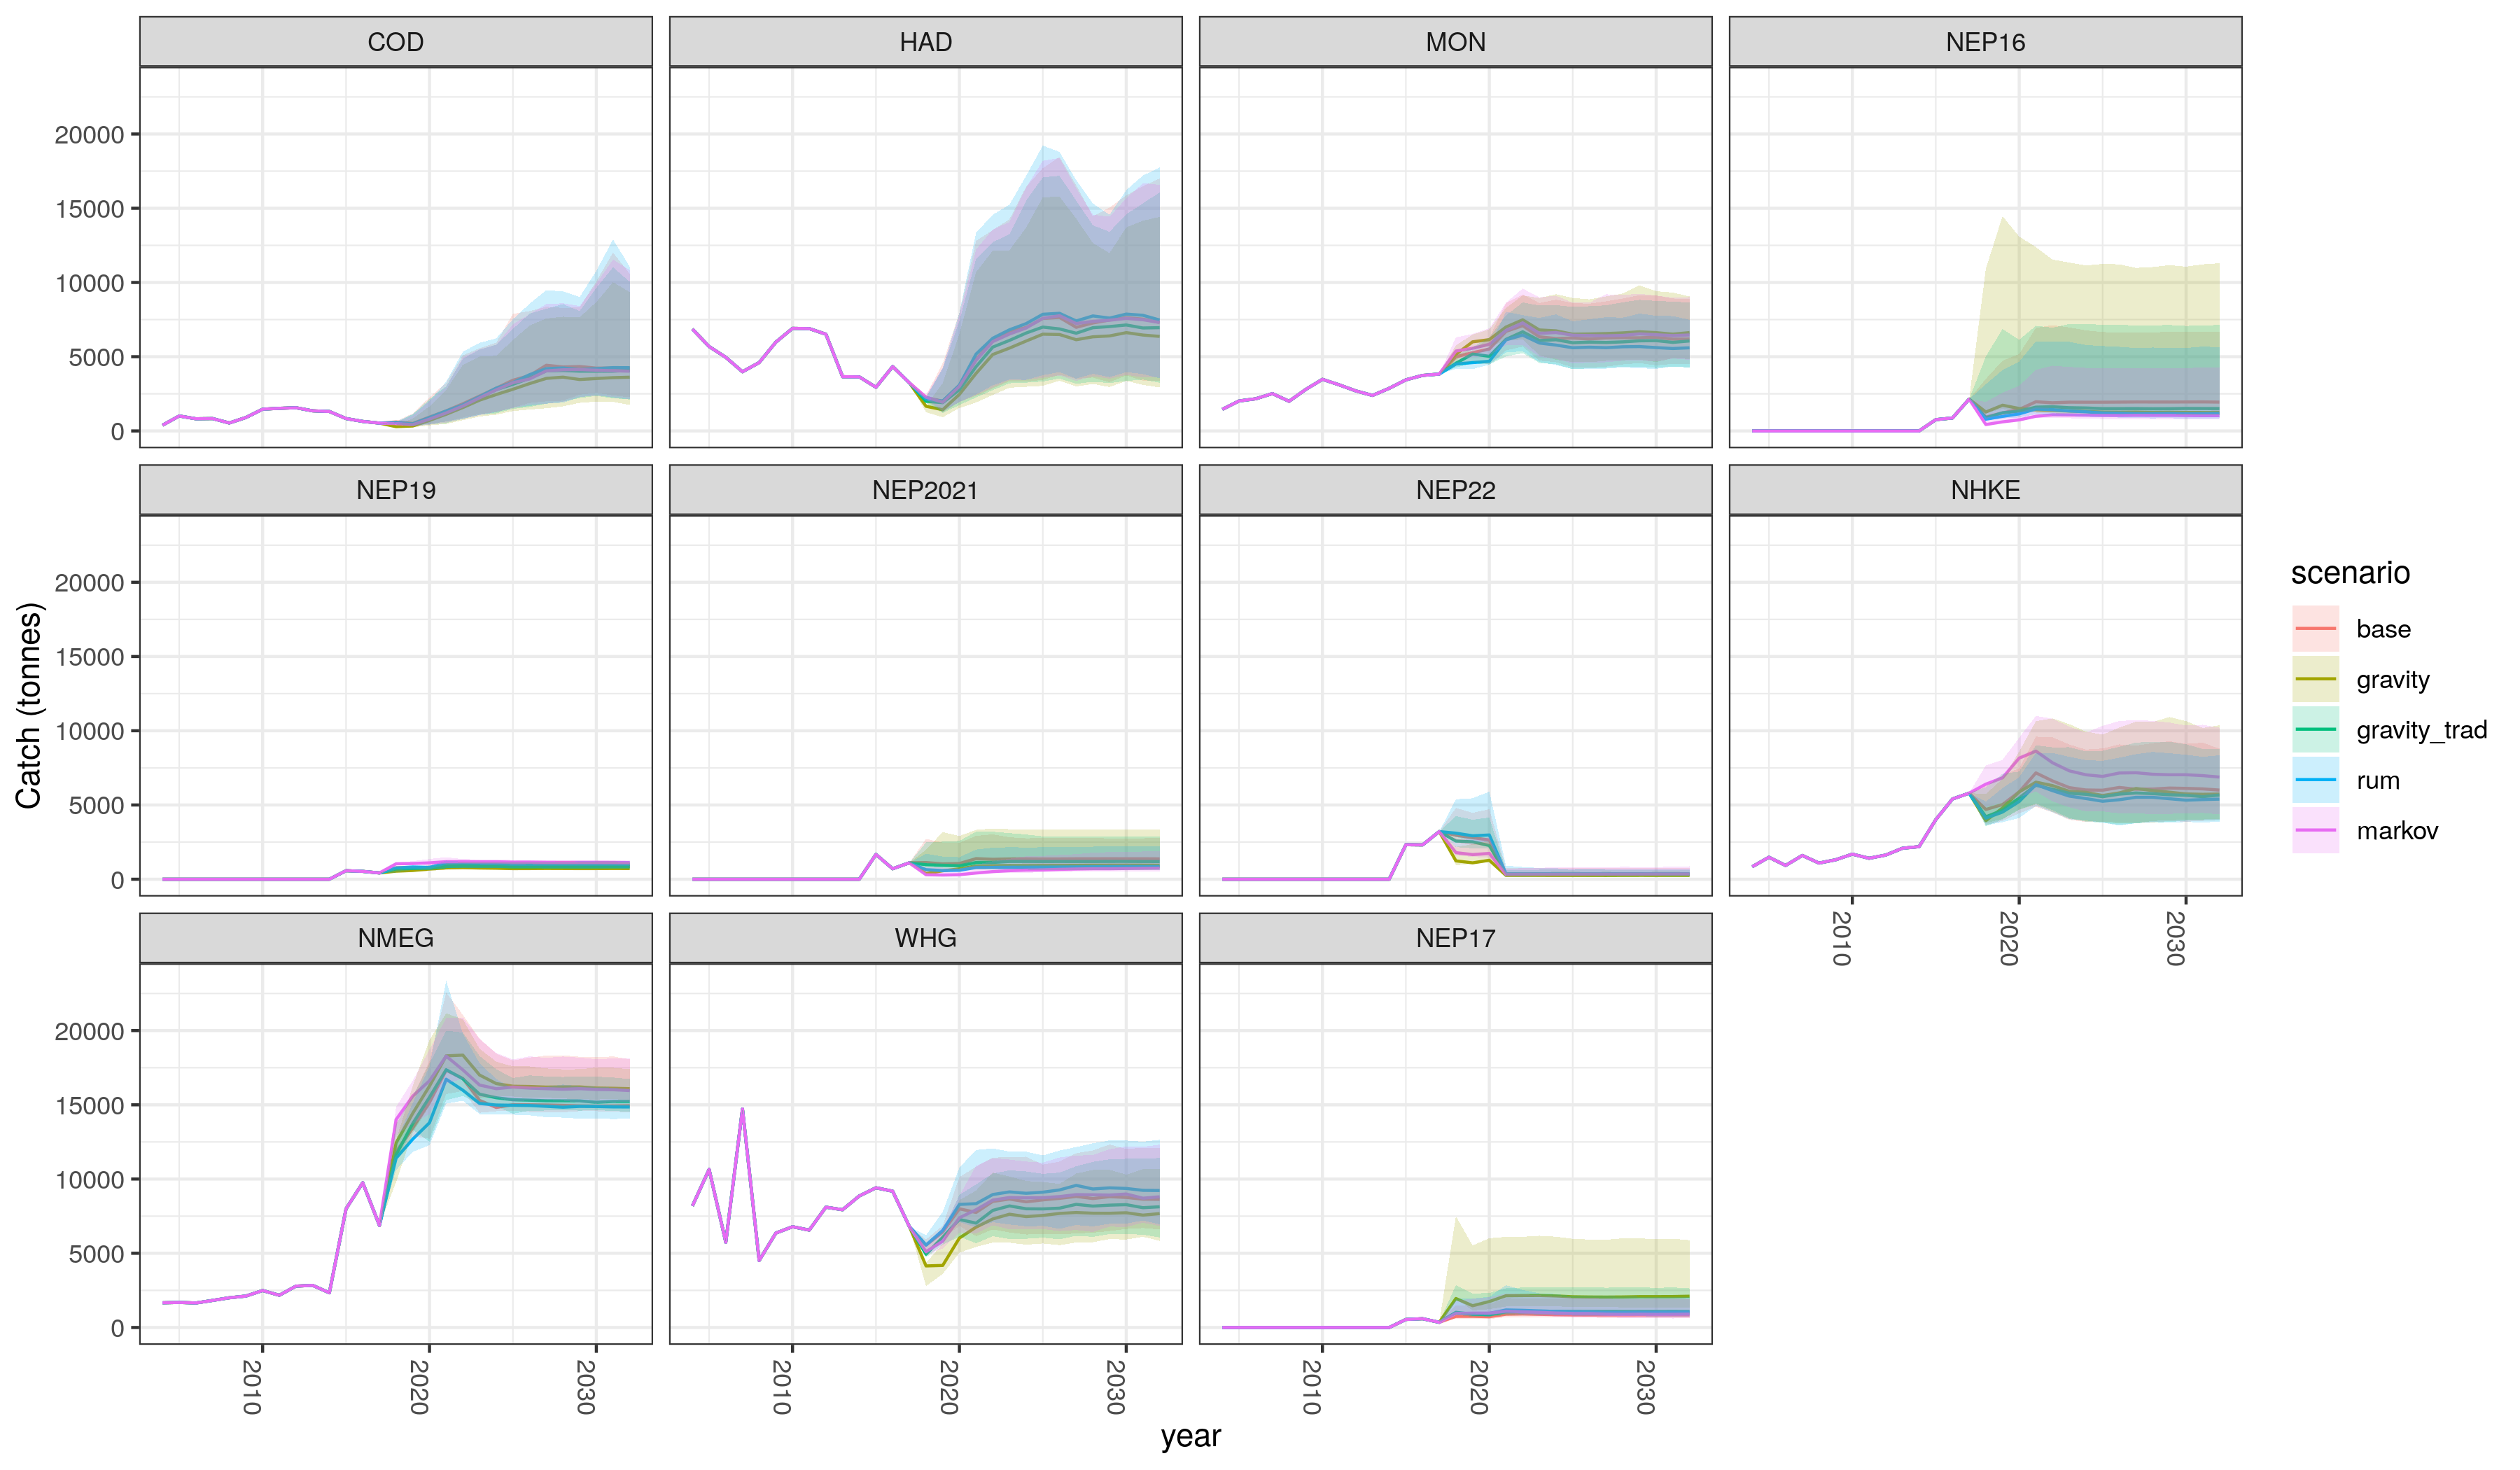
\includegraphics[width=1\linewidth]{figures/IE_Otter_catches}
	\caption{Catches of each stock by Irish Otter trawlers under the
		different location choice models. Light shading represents 5\%
		and 95\% variability due to recruitment and catchability. Solid
		line indicates end of the data/start of simulations and the
		dashed line the implementation of the spatial closure.} 
	\label{fig:OtterC}
\end{figure}	

\begin{figure}[!ht]
	\centering
	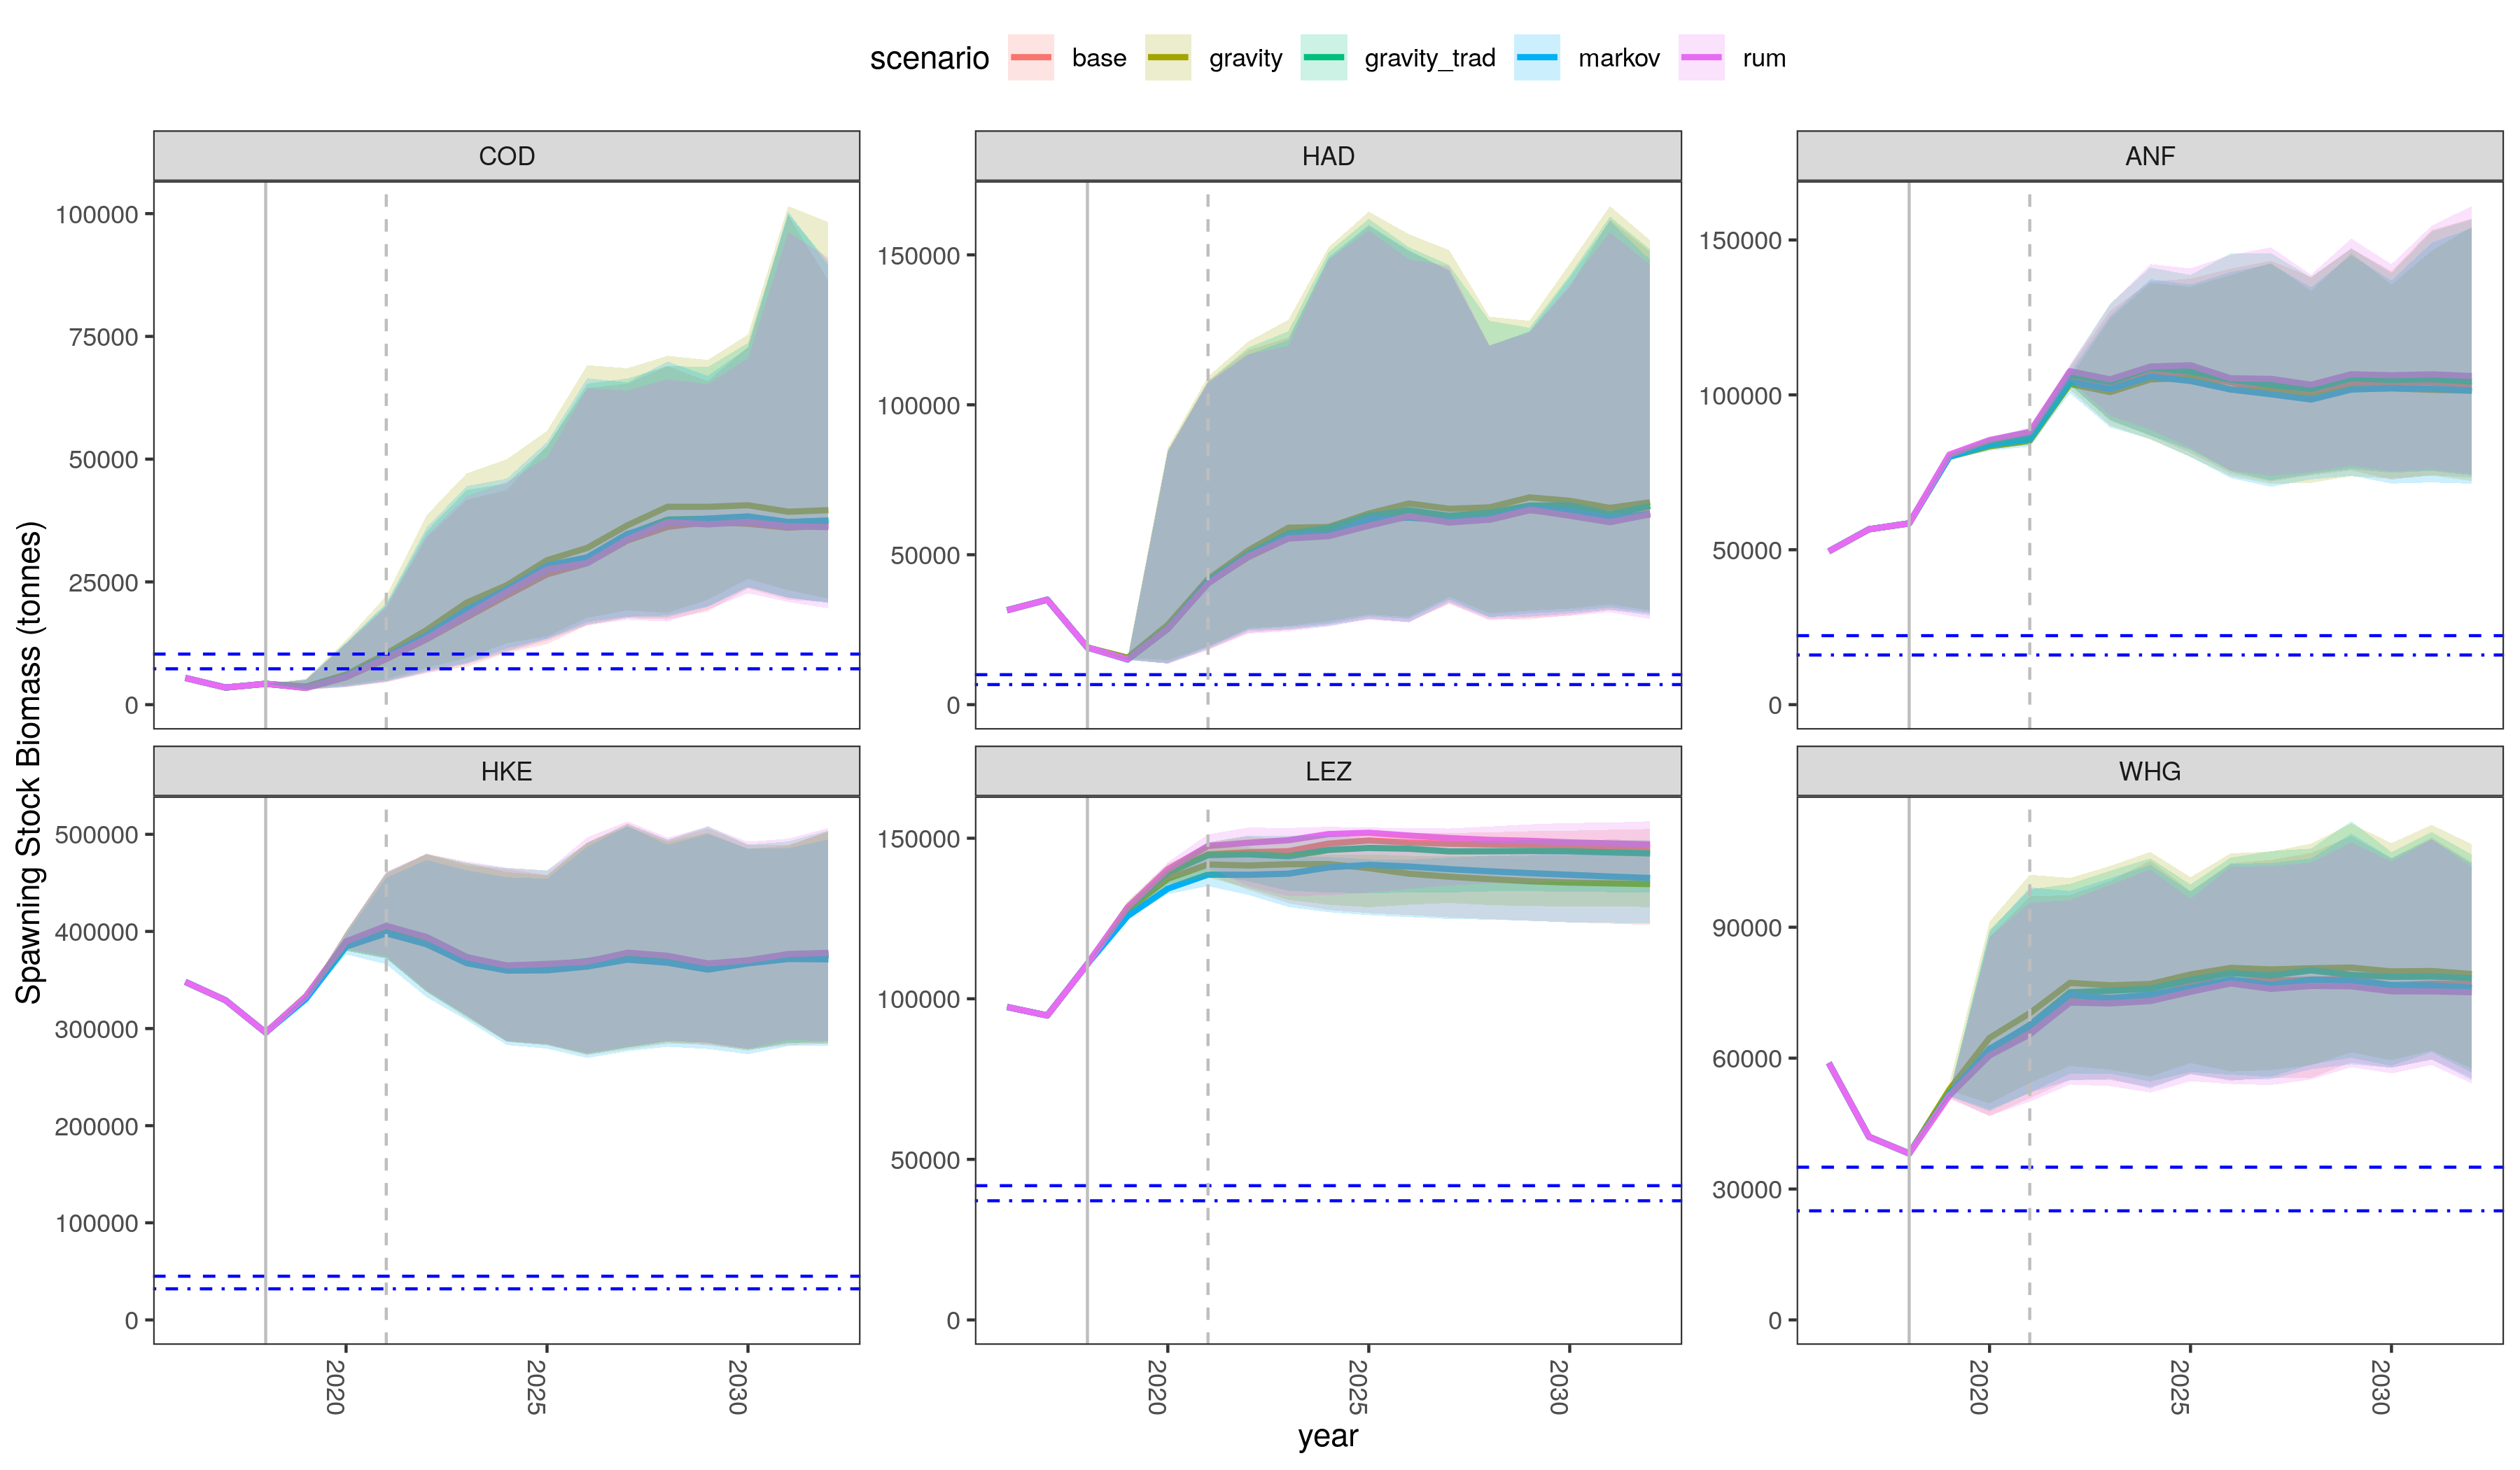
\includegraphics[width=1\linewidth]{figures/SSB_difference}
	\caption{Spawning Stock Biomass for the fish stocks under each location
		model scenario. Light shading represents 5\% and 95\%
		variability due to recruitment and catchability. Solid line
		indicates end of the data/start of simulations and the dashed
		line the implementation of the spatial closure.  Dotdashed and
		dashed blue lines indicate the Blim reference and Btrigger
		reference points respectively.} 
	\label{fig:SSB}
\end{figure}	

\begin{figure}[!ht]
	\centering
	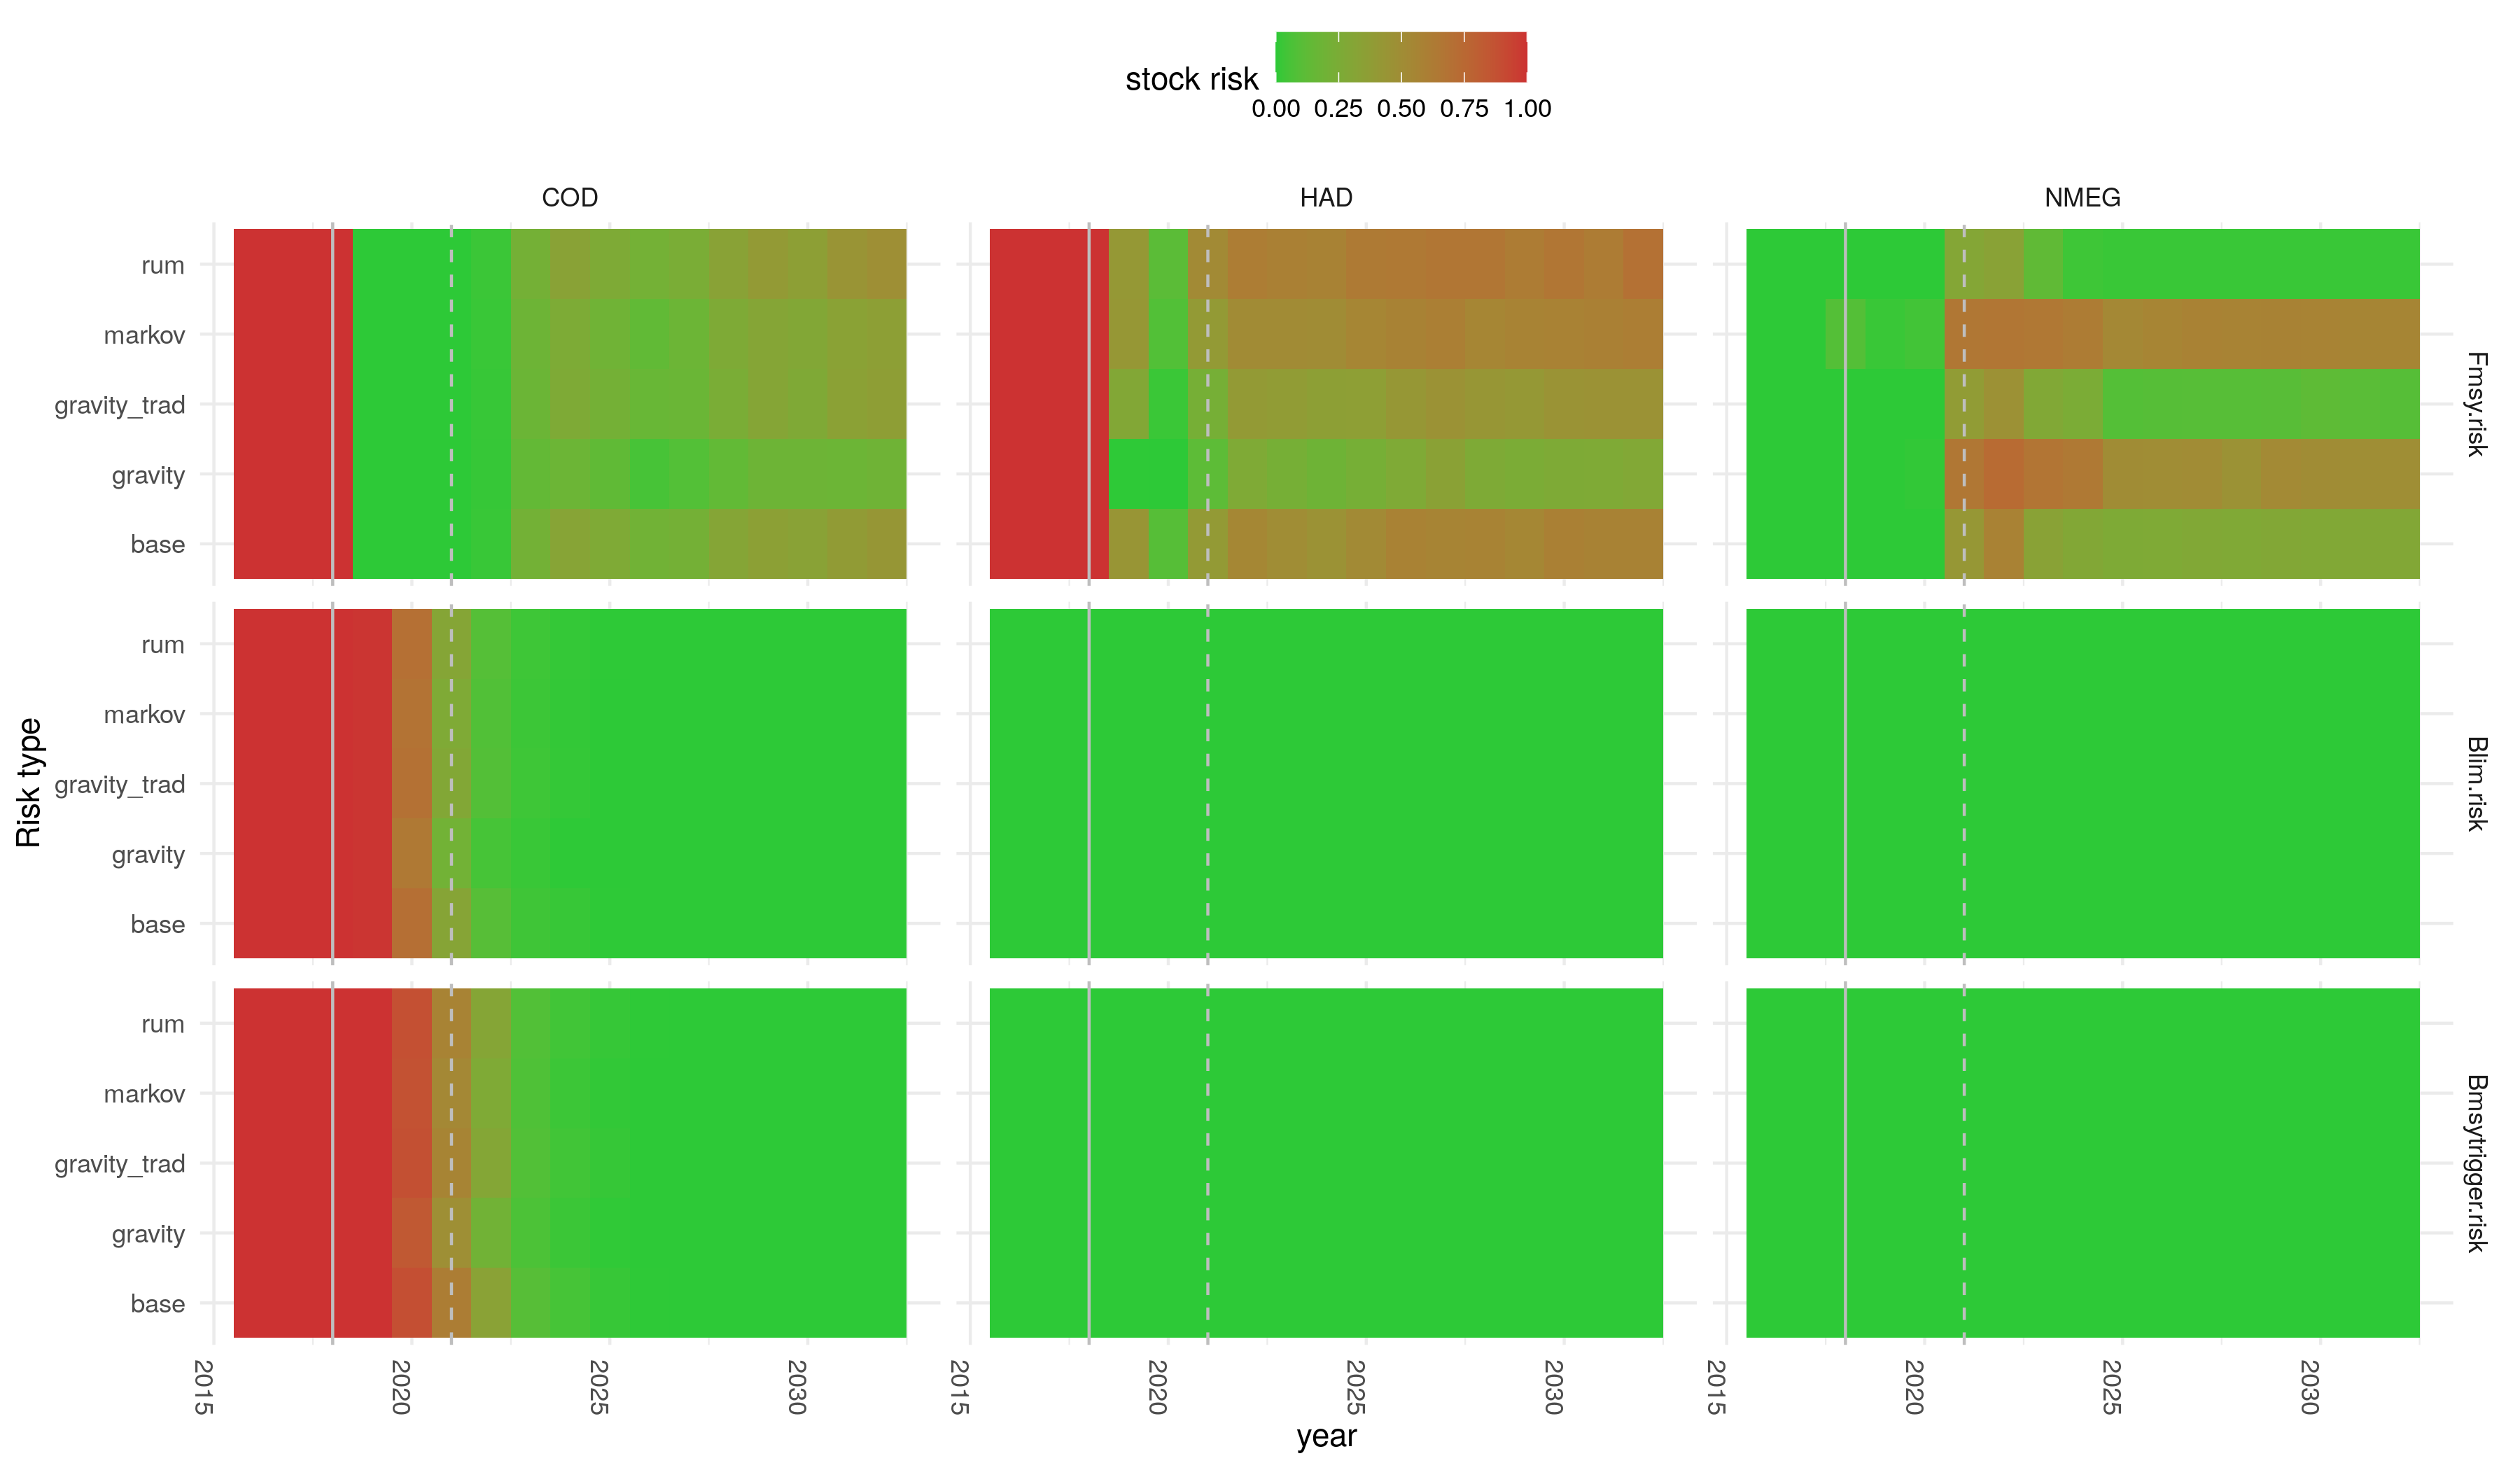
\includegraphics[width=1\linewidth]{figures/stock_risks}
	\caption{Stock risk indicators for each of the fish stock and location
		choice model scenarios. Solid
		line indicates end of the data/start of simulations and the
		dashed line the implementation of the spatial closure.} 
	\label{fig:risk}
\end{figure}	

%%%%%%%%%%%%%%%%%%%%%%%%%
\end{document}
